% #############################################################################
% This is Chapter 4
% !TEX root = main.tex
% #############################################################################
% Change the Name of the Chapter i the following line
\fancychapter{Annotating Lesion Contours}
\clearpage
% The following line allows to ref this chapter
\label{chap:chap004}

\ac{DL} algorithms (Section~\ref{sec:sec003007}) have increased the quality of automatic medical diagnosis at the cost of building datasets~\cite{10.1145/3313831.3376219} to train and test (Section~\ref{sec:sec003008}) such supervised \ac{ML} methods~\cite{10.1145/3206505.3206555}.
In the \ac{RRR} (Section~\ref{sec:sec002005}), medical imaging annotations~\cite{10.1145/3132272.3134111, calisto2019itmedex} are one of the main activities of radiologists and the quality of annotation depends on the clinician experience, as well as on the number of studied cases~\cite{doi:10.1148/radiol.2016150409}.
Manual annotations~\cite{10.1145/3399715.3399744} are very useful to extract features (Section~\ref{sec:sec002006}) like contours, intersections, margins, and shapes (Section~\ref{sec:sec002004}) that can be used in the processes of lesion segmentation (Section~\ref{sec:sec003007001}), {\it i.e.}, masses (Section~\ref{sec:sec002004001}) and microcalcifications (Section~\ref{sec:sec002004002}), as well as classification (Section~\ref{sec:sec003007002}), {\it i.e.}, \ac{BI-RADS}, made by intelligent agents~\cite{10.1145/3290605.3300468}.
In this chapter (Chapter~\ref{chap:chap004}), the document proposes~\cite{10.1145/3399715.3399744, https://doi.org/10.13140/rg.2.2.14792.55049, https://doi.org/10.13140/rg.2.2.16086.88649} a new framework that generate a standardized~\cite{lencastre2020mvf, calisto2015aqmgasa} dataset of medical imaging annotations, across the domain of breast cancer, adopting a multimodality strategy ({\it i.e.}, \ac{MG}, \ac{US} and \ac{MRI}) in order to provide clinicians a tool for the production of qualified datasets.
Also, this chapter will foster clinicians' sharing and collaborative (Section~\ref{sec:sec004002003}) evaluation by developing a distributed, remote accessible (Section~\ref{sec:sec004002004}) framework.

\section{Introduction}
\label{sec:sec004001}

In the context of breast cancer, the requirements for multimodality have a significant impact on the clinical workflow.
Although \ac{MG} is the primary imaging modality for breast screening, it may be insufficient to reach a correct and complete dataset generation for the intelligent agents and autonomous diagnostic purposes.
Therefore, support for visualization of multi-modal images and with associated dataset of annotations can provide improvements and insights in the breast screening radiology workflow.

With this document, the goal of this chapter is to propose a novel framework for the medical annotation of these lesion masses (Section~\ref{sec:sec002004001}) and microcalcifications (Section~\ref{sec:sec002004002}).
From the interaction between clinicians and this framework, a standardized dataset is generated.
Latter, this dataset will be consumed by the \ac{AI} algorithms.
On a multimodality visualization of medical images, the clinicians just need to delineate the contours of each lesion, in the presence of a mass.
Or just need to mark, by pointing, where the calcifications on the image are.
In the end, by consuming this data, the \ac{AI} algorithms can take into advantage the future integration of intelligent agents.
Thereafter, the intelligent agents are serving clinicians as a second reader opinion.

In order to annotate the medical images, the \ac{UI} comprises two lesion tools:
(1) a freehand polygon tool for annotating the masses of breast cancer lesions; and
(2) a bullet probe on the image for annotating the calcifications of breast cancer lesions.
These tools generate a dataset of manual annotations, which will be able to extract features ({\it e.g.}, lesion contours, intersections, and shapes) that can be used in the lesion segmentation and classification made by intelligent agents.
Such agents can have the integration of algorithms from \ac{AI}, \ac{ML} or \ac{DL} literature.

\section{Related Work}
\label{sec:sec004002}

Relevant for the current research, in this section the document identifies the literature related works and explain the advantages and disadvantages of each work.
Under this thesis, the document approach covers the limitations of the works following described.
More specifically, how the thesis is able to deal with non-homogeneous data, which is comprising multi-modal images, classification ({\it i.e.}, \ac{BI-RADS} score) and annotations ({\it i.e.}, delineation of the lesion contours).
To ascertain the usefulness of such non-homogeneous and multi-modal source of data, we aim to provide a novel solution for the lesion delineation.

\subsection{Raised Labeling Problems}
\label{sec:sec004002001}

\ac{AI}-assisted interfaces already showed breakthroughs in the clinical domain (or in this case, the breast cancer diagnosis), through high quality data ({\it i.e.}, the \ac{BI-RADS} classification provided by \ac{DL} methods) with annotations~\cite{https://doi.org/10.13140/rg.2.2.25412.68486}.
In part, the goal behind the thesis work is to integrate a \ac{CNN} for each modality ({\it i.e.}, \ac{CNN} channel), and then to perform a ``deep fusion'' over the different channels~\cite{liu2019sdfn, wei2019medical}.
This will allow the work to implement, integrate and use the learned high-level features of all channels.
Such channels are finding patterns on lesion masses and microcalcifications.
The training is  supervised, or semi-supervised~\cite{philbrick2019ril, zhao2019data, zhou2019collaborative}, meaning that the deep architecture will need the ground-truth (annotations and \ac{BI-RADS} classification) obtained via the support of a multimodality strategy~\cite{huang2019diagnosis, soffer2019convolutional}.
Therefore, the support for multi-modal \acp{UI}~\cite{gotz2019mitk, wels2019general} is a fundamental step in the development of such contributions.
This will also enable radiologists to intervene in the workflow, whenever a new image is added to the network.
In addition, the concept of  ``{\it aging the net}''~\cite{smailagic2019medal} is also reachable, meaning that a \ac{CNN} architecture can be fully supervised, trained as more examples are ready to be provided into the network.

\subsection{Cancer Detection and Diagnosis}
\label{sec:sec004002002}

Frequently used in cancer detection and diagnosis, \ac{ML} has been recently applied for cancer prognosis and prediction~\cite{KOUROU20158}.
In fact, the ability of \ac{ML} tools to detect key features from complex datasets reveals their importance.
This latter approach is particularly interesting as it is part of a growing trend towards personalized and predictive medicine.
At a more fundamental level, it is also evident that these tools are also helping to improve a basic understanding of cancer development and progression.
Several works are assembling this review~\cite{https://doi.org/10.1111/cen.12731, antonanzas2015some, hood2011predictive}, conducting a broad research for different types of used tools~\cite{Huang_2017_CVPR, 8515234, 10.1007/978-3-030-00934-2_99}, types of data being compared~\cite{MOREIRA2012236, 7813261, shen2019deep} and the characteristics of these tools in cancer predictions and prognosis~\cite{KOUROU20158, hood2011predictive}.
However, a number of studies~\cite{Cai:2019:HTC:3290605.3300234, 10.1167/tvst.8.6.40} are also appearing to lack on appropriate level of features to support the proposed tool for a standardized generation of a datasets with medical imaging annotations.
Making the contribution of this chapter so important.

Some contributions~\cite{10.1001/jamainternmed.2015.5231, jiang2018interpretation, 10.1145/3373017.3373051} are showing how the use of their \ac{CADe} systems can output different lesion displays.
Addressed in this chapter, the authors' ideas are followed for providing accurate representations of areas in subsequent exams.
Since the \ac{CADe} output is not used during the initial reading, the radiologist does not mark it until a final determination is reached.
Furthermore, \acp{ROI} are indicated in the context of a particular anatomical detail.
The work developed by Jalalian et al.~\cite{JALALIAN2013420} assists the technologist, other physicians and patients in more efficiently and accurately way, locating the exact area for subsequent exams.
The work presents several advantages and disadvantages in comparison to the proposed framework under this chapter.
First of all, the work is related and ready for both medical imaging technologies and is applied for the breast cancer domain.
Moreover, this work is ready for a multimodality strategy with lesion annotations on a remote fashion.
Despite the completeness of their solution, it does not provide a standardized generation of a dataset with medical imaging annotations.

\subsection{User Sharing and Collaboration}
\label{sec:sec004002003}

Nowadays, technology may miss significant and relevant cross information between clinicians~\cite{10.1145/3313831.3376710}.
Even though, when leading clinicians diagnose to their patients through several data recordings.
Concerning the above raised set of problems, during the literature review it was observed a lack of system features for sharing and collaborative tools that should be addressed.

Sargent et al.~\cite{10.1007/978-3-030-59725-2_21} are presenting a diagnosis support system providing automated guidance to a user by automated retrieval of similar disease images and user feedback.
High resolution standardized labeled and unlabeled, annotated and non-annotated images of diseased tissue in a database are clustered, preferably with expert feedback.
Similarly, several other contributions~\cite{10.3389/fphy.2018.00051, DALILA2017749} are offering the feature of lesion annotations on a clinical environment using medical imaging technologies.
However, these contributions are limited in other ways.
Most importantly, the contributions do not provide a sharing and collaborative tool between clinicians, as well as institutions.
Moreover, all of these contributions are not ready for a multimodality strategy of a breast cancer diagnosis.

\subsection{Distributed and Remote Accessible}
\label{sec:sec004002004}

In this section, the thesis takes into consideration a set of contributions.
Regarding the available literature of remote and diagnostic systems in medical imaging, several works are addressed.
Here, the document addresses the several contributions, while demonstrating what are the advantages and disadvantages in comparison to the proposed framework in this chapter.
For instance, the work developed by Schaekermann et al.~\cite{10.1167/tvst.8.6.40} is presenting and evaluating a remote, tool-based system and structured grading rubric for adjudicating (Section~\ref{sec:sec003005}) image-based diabetic retinopathy grades~\cite{10.1145/3359178}.
However, their tool is not prepared trivially for breast cancer diagnostic.

In the work developed by Sirintrapun et al.~\cite{10.1200EDBK200141}, the authors have studied telemedicine uses of telecommunications technology as a tool to deliver better patient care in populations with limited access to care.
Simirlarly, works like Li et al.~\cite{10.1007/978-3-319-59050-9_28} and Gibson et al.~\cite{GIBSON2018113} contributed for the development of the \href{https://github.com/NifTK/NiftyNet}{NiftyNet}\footnotemark[11] platform, an open-source platform for \ac{DL} in medical imaging.
The authors did a great work, developing a solid and useful tool for the community.
However, the tool relies on segmentation methods of multiple abdominal organs, brain \ac{MRI} volumes, and \ac{US} images for specified anatomical poses, not much prepared for the breast typical use cases.
Moreover, the tool does not provide any classification functionality, which make it impossible to properly classify the image and each type of potential lesions.
Making it unsuitable for breast cancer purposes ({\it e.g.}, a functionality for lesion annotations of masses or microcalcifications is missing) and, therefore, the main motivation to the development of a new framework such as the one presented in this chapter.

%%%%%%%%%%%%%%%%%%%%%%%%%%%%%%%%%%%%%%%%%%%%%%%%%%%
\footnotetext[11]{\href{https://github.com/NifTK/NiftyNet}{NiftyNet} (\href{https://niftynet.io/}{niftynet.io}) is a \href{https://www.tensorflow.org/}{TensorFlow}-based open-source \ac{CNN} platform for research in medical image analysis and image-guided therapy. The platform modular structure is designed for sharing networks and pre-trained models. The links were assessed in November 2020.}
%%%%%%%%%%%%%%%%%%%%%%%%%%%%%%%%%%%%%%%%%%%%%%%%%%%

\section{Framework Details}
\label{sec:sec004003}

In conjunction with the following figures and diagrams, it will be better understood the specific embodiment of the presented framework.
In this section, the document describe a more complete understanding of the available functionalities and advantages for the proposed tool.
In this thesis, a tool called {\it BreastScreening} was designed under the following framework technical specifications.
While making and using various embodiment items, the framework characteristics and tool design are discussed in detail below.
As appreciation, the presented contribution provides many applicable concepts that can be embodied in a wide variety of medical imaging contexts.
The specific embodiment items are discussed herein and are merely illustrative of specific ways to make and use the framework, not limited to the scope of the breast domain.

\subsection{User Interface}
\label{sec:sec004003001}

For this framework and consequent design of a tool within the purpose of annotating breast cancer lesions and patient classification, the \ac{UI} consists of two main components:
{\it 4. List of Patient Views}; and
{\it 5. Medical Imaging Diagnosis Views}.
These two main components (Figure \ref{fig:fig003} and Figure \ref{fig:fig028}) are also divided into several sections:
{\it 4.1. List of Patients};
{\it 4.2. Header};
{\it 4.3. Help};
{\it 4.4. About};
{\it 4.5. Study List Tabs};
{\it 5.1. Viewports};
{\it 5.2. Toolbars}; and
{\it 5.3. Modality Selection}.
The first tool view is the {\it 4. List of Patients Views}.
With this view, clinicians can quickly choose the respective {\it 4.1. List of Patients}.
Using the \ac{BI-RADS} functionality ({\it 6.3.1.~Physician Severity}), clinicians can now classify (Figure \ref{fig:fig003}) the severity of the breast lesion for each patient.

%%%%%%%%%%%%%%%%%%%%%%%%%%%%%%%%%%%%%%%%%%%%%%%%%%%
\begin{figure}[ht]
\centering
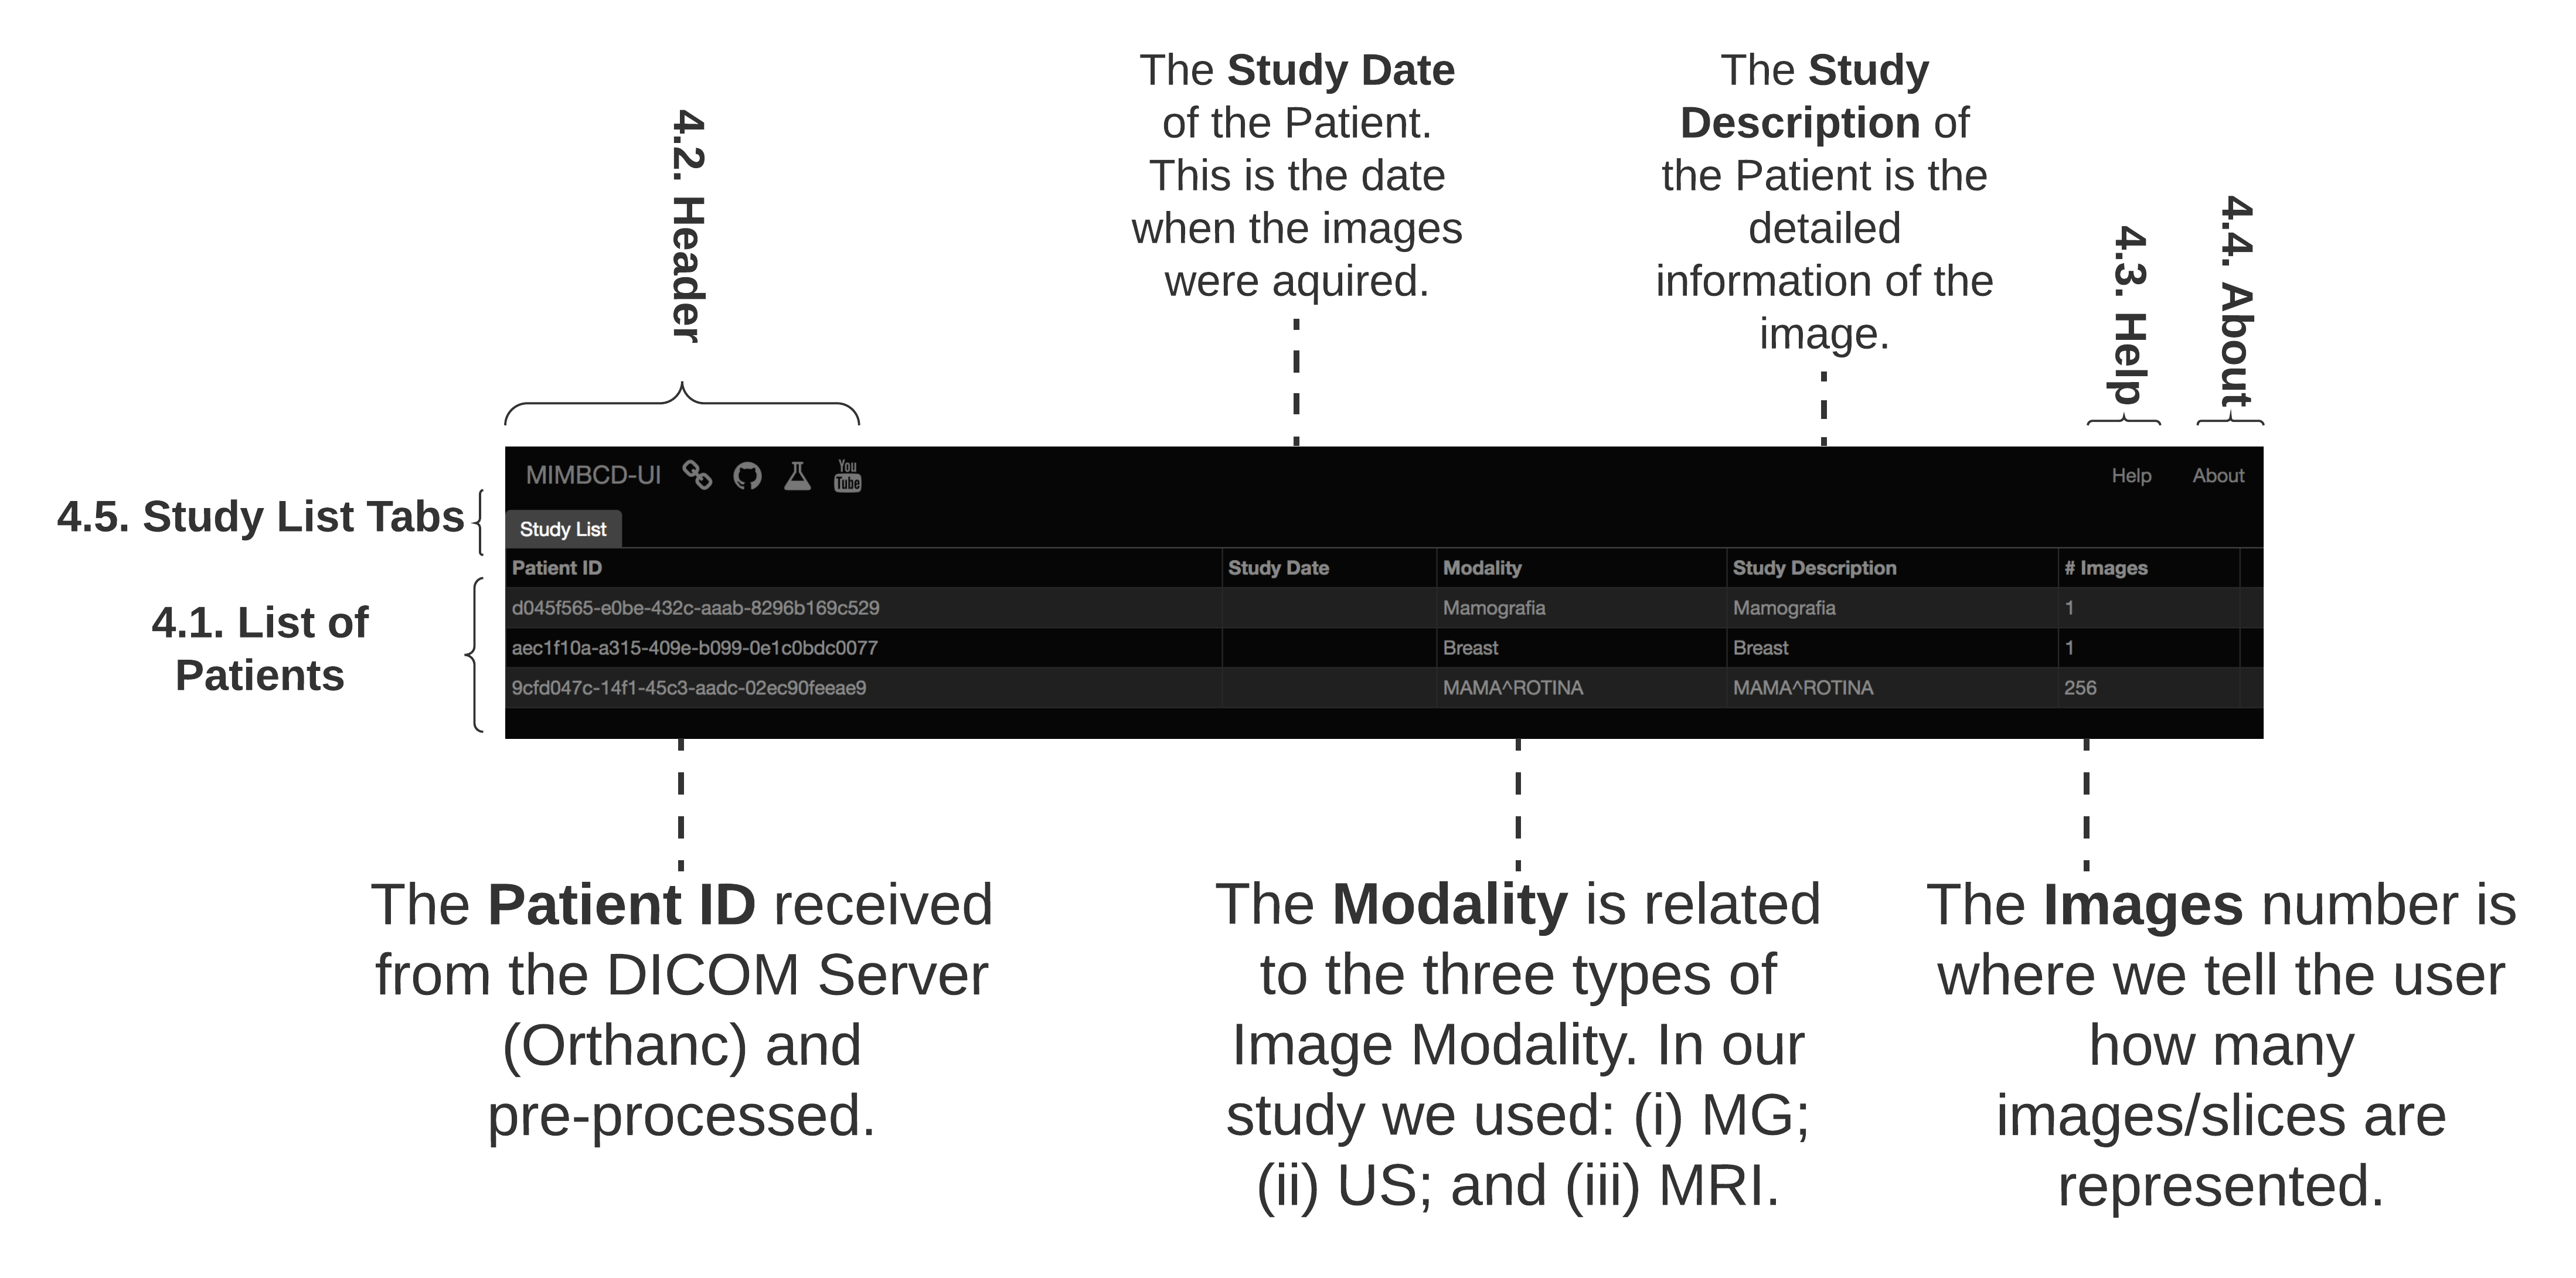
\includegraphics[width=\textwidth]{images/fig003}
\caption{{\it BreastScreening} provides clinician support to easily access and switch between the patient views. When accessing the assistant, the first screen shows the list of patients. Each row of the table, represents a patient. Each patient has a {\bf Patient ID}, {\bf Study Date}, {\bf Modality} (one or more), {\bf Study Description} and number of {\bf Images}.}
\label{fig:fig003}
\end{figure}
%%%%%%%%%%%%%%%%%%%%%%%%%%%%%%%%%%%%%%%%%%%%%%%%%%%

\subsubsection{List of Patients}
\label{sec:sec004003001001}

The first information (Figure~\ref{fig:fig003}) pointed by clinician (Chapter~\ref{chap:chap005}) is the {\it 4. List of Patient Views} so that the clinician can quickly choose the respective {\it 4.1. List of Patients} for the task for classifying ({\it i.e.}, providing the \ac{BI-RADS}) the breast severity of each patient.
This {\it 4.1. List of Patients} contains the most important and needed information avoiding the excess of information typically presented on these systems.

Compared to early developments~\cite{10.1145/3132272.3134111, calisto2017mimbcdui}, the tool potentially improved the temporal awareness (Chapter~\ref{chap:chap005}) of the \ac{RRR} with the introduction of these functionalities.
The {\it 4.2. Header} represents a shortcut to the {\it 4.1. List of Patients}.
Also, if a clinician needs some support ({\it e.g.}, domain questions), providing both {\it 4.3. Help} and {\it 4.4. About} components on the \ac{UI} is giving clinicians' the information of how to proceed.
For instance, these components were used mainly by Intern\footnotemark[12] clinicians, where they took advantage of this information gaining time over diagnostic.
The {\it 4.5. Study List Tabs} gives the clinicians' opportunity to switch between the patient who is being diagnosed and the next patient to be open.

%%%%%%%%%%%%%%%%%%%%%%%%%%%%%%%%%%%%%%%%%%%%%%%%%%%
\footnotetext[12]{The medical professional experience of clinicians was divided across the following categories: (1) Seniors - more than 10 years of medical practical experience; (2) Middles - more than 5 years but less than 10 years of medical experience; (3) Juniors - after taking the exam, up to 5 years of medical experience; and (4) Interns - limited medical experience.}
%%%%%%%%%%%%%%%%%%%%%%%%%%%%%%%%%%%%%%%%%%%%%%%%%%%

During the patient diagnosis (Section~\ref{sec:sec002005002}) stage, each clinician selects one patient to perform the diagnostic.
Then, a window will open the respective patient and the clinician can start manipulating the image according to a specific criteria.
At this point the clinician can make two choices: (1) opens the image by dragging to the view-port; or (2) select the provided tools before opening the image.

Given this set of tools, the developed framework is now equalizing the actual hospitals system in terms of functionalities.
Moreover, the tool is improving the temporal awareness of clinicians in many clinical use cases.
With this designed tool, not only the framework is giving the same number of needed functionalities to clinicians, but also providing researchers the opportunity to query clinicians' annotations and classifications remotely.
Although, several functionalities were studied and are already being develop leading space for more workflow improvements.
By providing future functionalities (Chapter~\ref{chap:chap008}), clinicians be able to do more in less time, which will influence the quality of the final annotations and classifications.

%%%%%%%%%%%%%%%%%%%%%%%%%%%%%%%%%%%%%%%%%%%%%%%%%%%
\begin{figure}[ht]
\centering
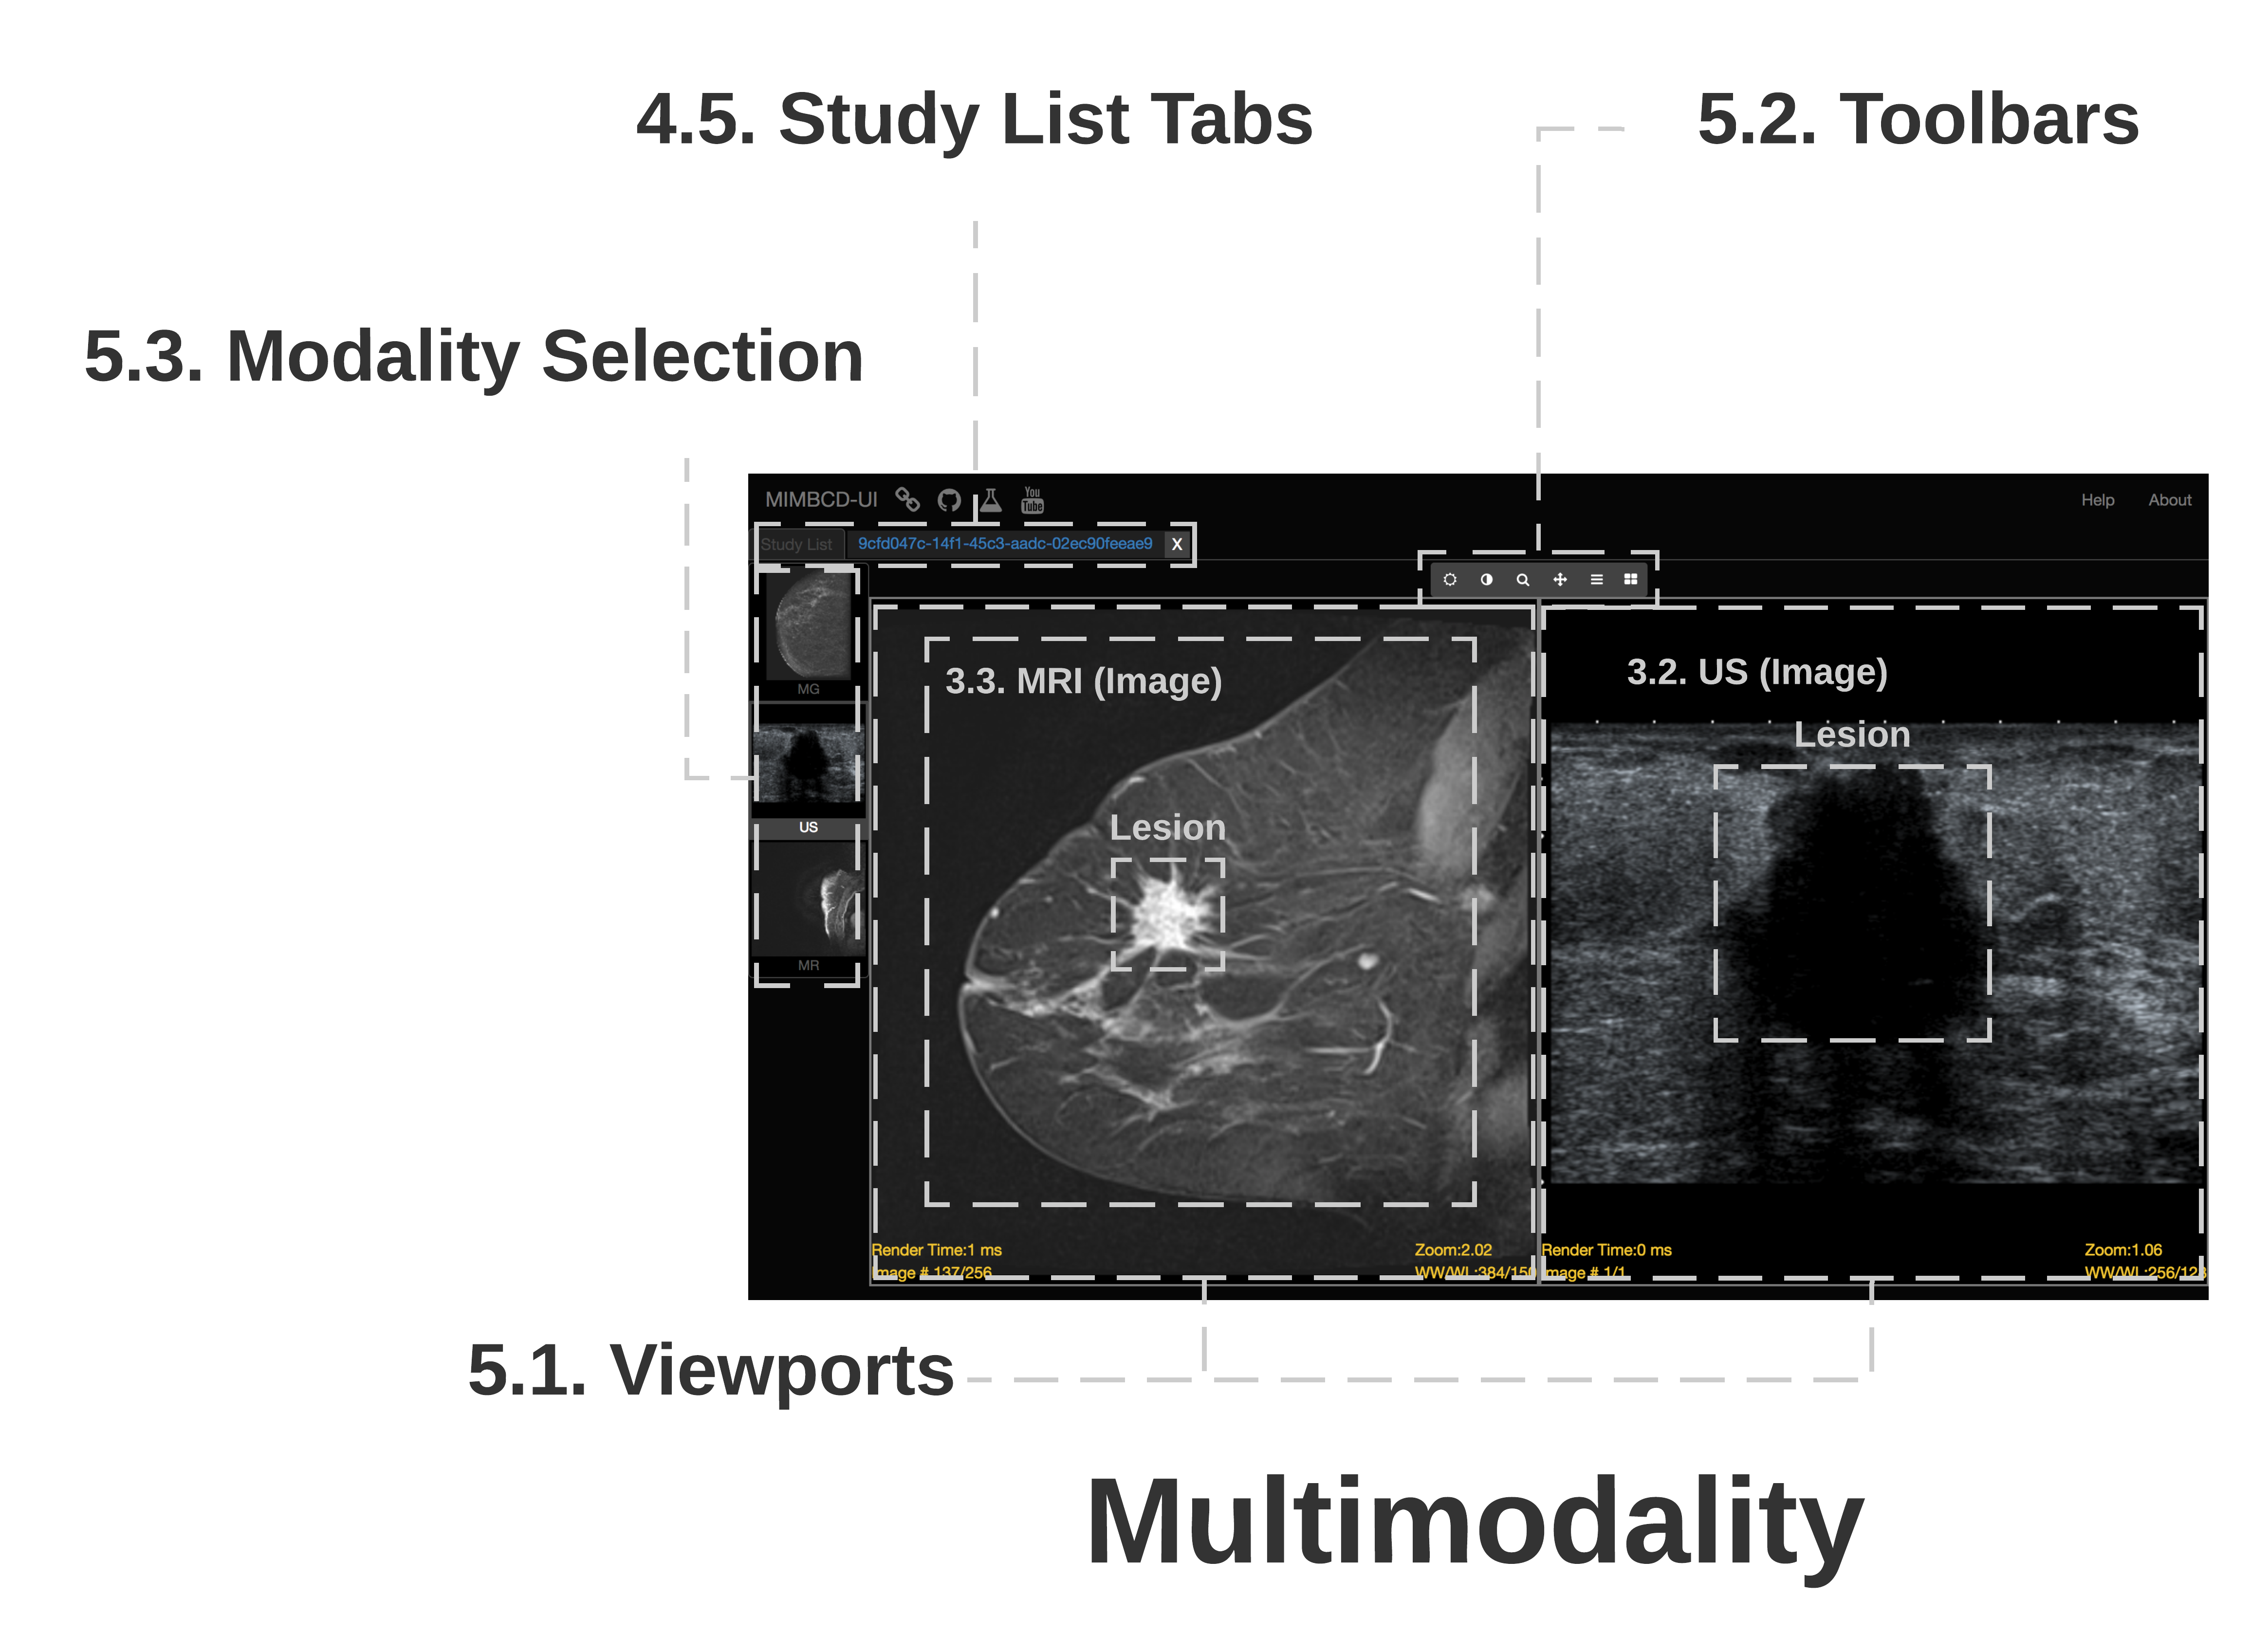
\includegraphics[width=\textwidth]{images/fig028}
\caption{The multimodality view of the framework and designed tool. The UI components are as follows: {\it 4. List of Patient Views}; and {\it 4.5. Study List Tabs}; as well as {\it 5. Medical Imaging Diagnosis Views}; {\it 5.1. Viewports}; {\it 5.2. Toolbars}; and {\it 5.3. Modality Selection}.}
\label{fig:fig028}
\end{figure}
%%%%%%%%%%%%%%%%%%%%%%%%%%%%%%%%%%%%%%%%%%%%%%%%%%%

\subsubsection{Medical Imaging Diagnosis}
\label{sec:sec004003001002}

In the last section, the document introduced the concept of {\it 4.1. List of Patients} for the patient diagnostic task.
In this section, the document is introducing the concept of {\it 5. Medical Imaging Diagnosis Views} (Figure~\ref{fig:fig028}) from the designed tool.
As follows, more details are describing each functionality.

Concerning the point {\it 5. Medical Imaging Diagnosis Views}, the component is mainly supported by the management of viewports, set of toolbars and modality selection.
As already said, this component is contributing for the temporal awareness\footnotemark[13] of each clinician by providing other functionalities.
More specifically, the clinician can probe for lesion patterns via the {\it 5.1. Viewports} functionality and processing the image by using the {\it 5.2. Toolbars} (Figure~\ref{fig:fig008}) functionalities.

Each time the {\it 5.2. Toolbars} functionalities are activated, the clinician needs to perform a simple and easy interaction with the medical image to configure it as desired.
Using the {\it 5.2. Toolbars} (Figure~\ref{fig:fig008}) on the {\it 5.1. Viewports}, the clinician can locate the lesions and classify the lesions severity (\ac{BI-RADS}).
Furthermore, {\it 5.2. Toolbars} (Figure \ref{fig:fig028}) were positioned so as to correspond the clinician's expectations, an outcome of the observations and interviews phases.

%%%%%%%%%%%%%%%%%%%%%%%%%%%%%%%%%%%%%%%%%%%%%%%%%%%
\footnotetext[13]{A statistical analysis was published regarding those values. For that, internet connection is needed to have access to it. The statistical data page (\href{https://mimbcd-ui.github.io/statistical-analysis/mm_measures_time_vs_clicks.html}{mimbcd-ui.github.io/statistical-analysis}) was accessed on the 30th of November, 2020.}
%%%%%%%%%%%%%%%%%%%%%%%%%%%%%%%%%%%%%%%%%%%%%%%%%%%

\subsubsection{Toolbars}
\label{sec:sec004003001003}

Current functionalities (Figure~\ref{fig:fig008}) for image processing are including:
{\it 5.2.1. WW/WC} (Window Width/Window Contrast);
{\it 5.2.2. Invert};
{\it 5.2.3. Zoom};
{\it 5.2.4. Pan};
{\it 5.2.5. Stack-Scroll};
{\it 5.2.6. Windows};
{\it 5.2.7. Freehand};
{\it 5.2.8. Probe}; and
{\it 5.2.9. Save}.
These functionalities are included on the multimodality views (Figure~\ref{fig:fig028}) of developed framework.

%%%%%%%%%%%%%%%%%%%%%%%%%%%%%%%%%%%%%%%%%%%%%%%%%%%
\begin{figure}[ht]
\centering
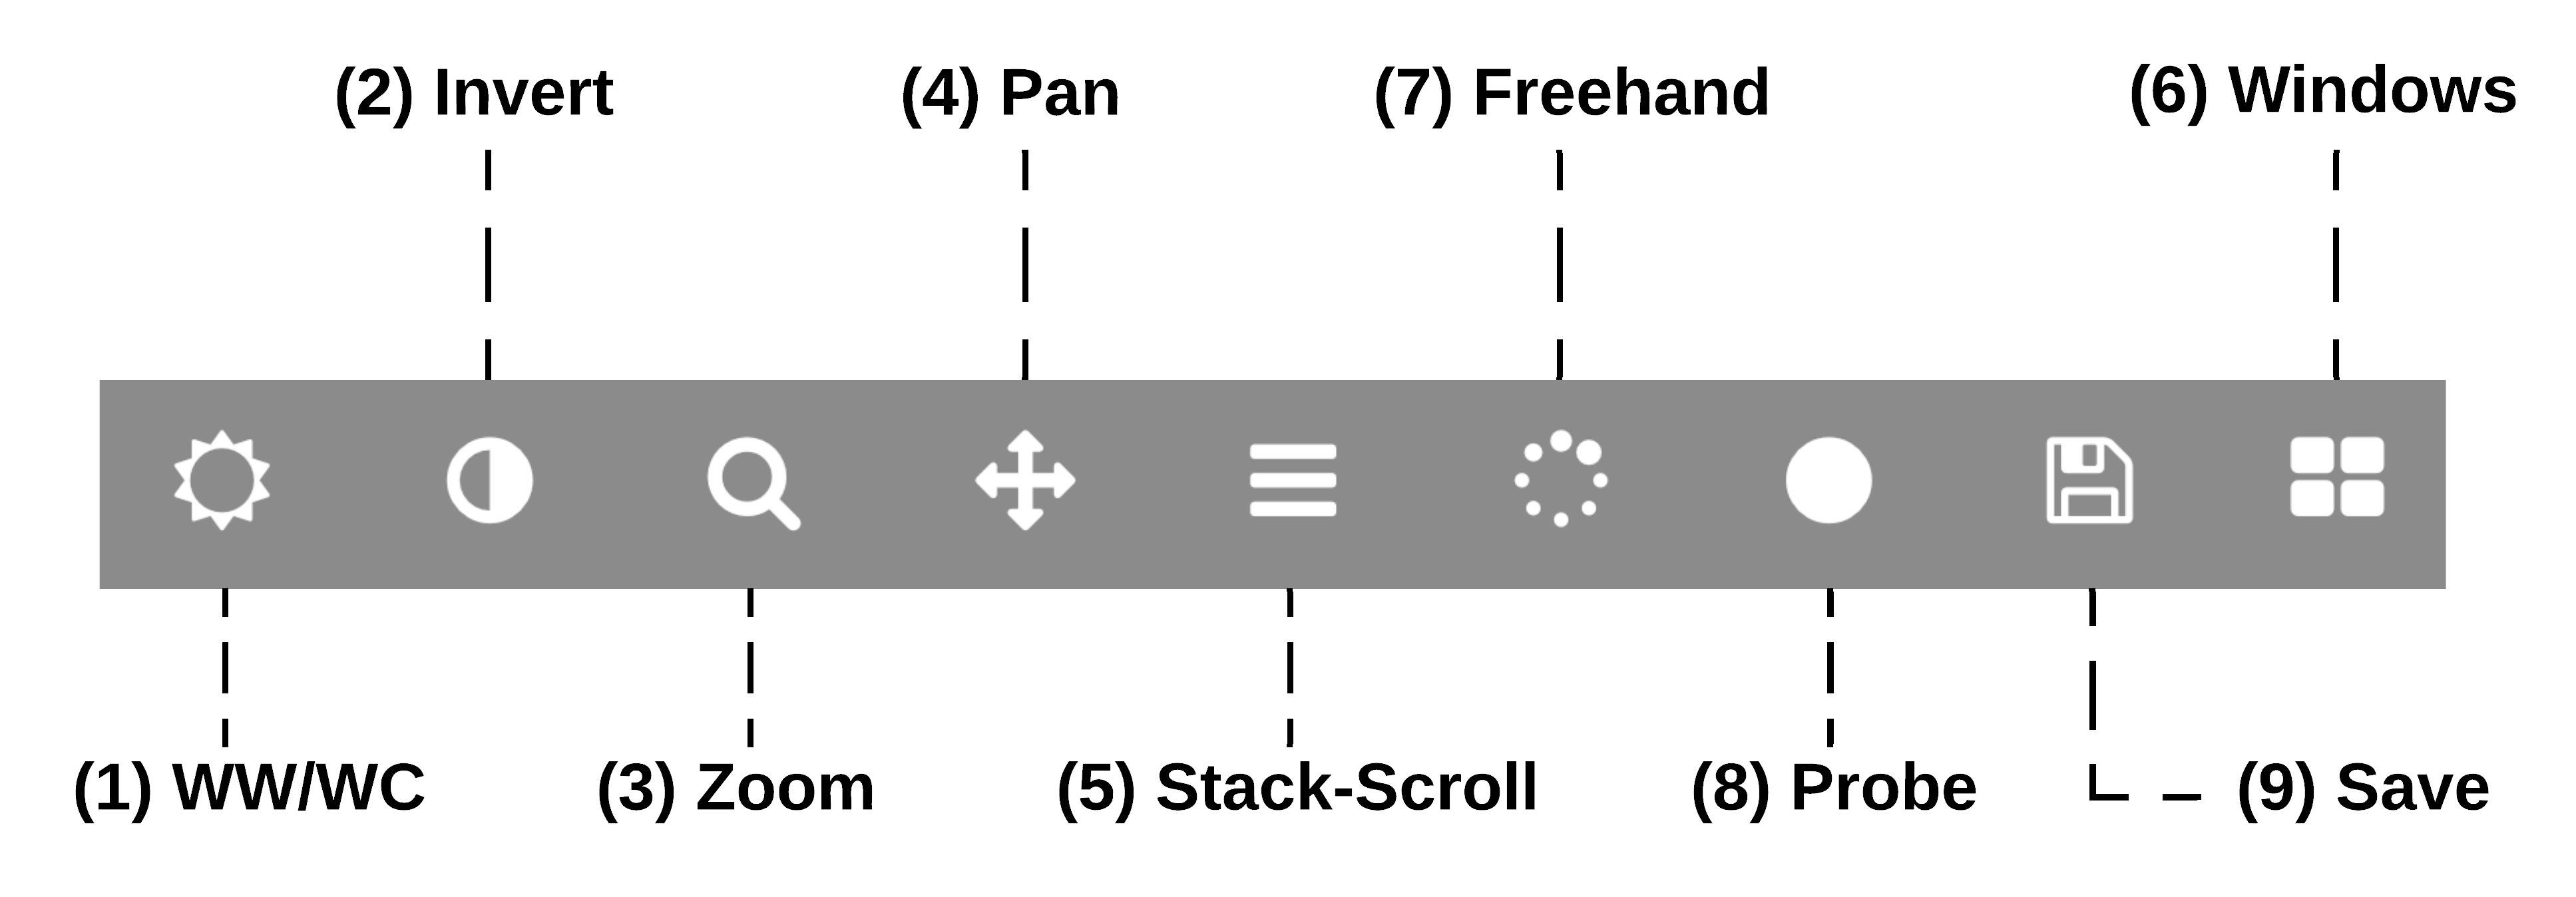
\includegraphics[width=\textwidth]{images/fig008}
\caption{The {\it 5.2. Toolbars} of the developed framework and designed tool. Currently, the available features are: {\it 5.2.1. WW/WC}; {\it 5.2.2. Invert}; {\it 5.2.3. Zoom}; {\it 5.2.4. Pan}; {\it 5.2.5. Stack-Scroll}; {\it 5.2.6. Windows}; {\it 5.2.7. Freehand}; {\it 5.2.8. Probe}; and {\it 5.2.9. Save}.}
\label{fig:fig008}
\end{figure}
%%%%%%%%%%%%%%%%%%%%%%%%%%%%%%%%%%%%%%%%%%%%%%%%%%%

The contrast and brightness can be adjusted by selecting the {5.2.1. WW/WC} option on the {\it 5.2. Toolbars} and then left-clicking over the image configuring it by moving the mouse at the same time.
The same interaction technique is applied for {\it 5.2.3. Zoom}, {\it 5.2.4. Pan} and  {\it 5.2.5. Stack-Scroll}.
To invert the pixels of the image, user just needs to select the (2) {\it 5.2.2. Invert} on the {\it 5.2. Toolbars}.
The {\it 5.2.6. Windows} will open a drop-down list of possible viewport designs ({\it i.e.}, $1\times 1$, $2\times 1$, $1\times 2$ and $2\times 2$).

In this chapter, the document focus on the delineation of lesion contours (Section~\ref{sec:sec004003002001}) and respective generation of the annotations (Section~\ref{sec:sec004003002002}).
Notwithstanding, the lesion contours are concerning the masses and microcalcifications regarding the breast cancer disease.
On the same hand, the generation of annotations process is creating a standardized dataset and storing this information on a remote server.
That said, despite highly useful for the patient diagnostic and for the image segmentation (Section~\ref{sec:sec004003002002}), this chapter focus does not rely on the latter ({\it e.g.}, {\it 5.2.1. WW/WC}, {\it 5.2.2. Invert}, {\it 5.2.3. Zoom}, {\it 5.2.4. Pan}, {\it 5.2.5. Stack-Scroll} or {\it 5.2.6. Windows}) features.
Instead, we are focusing this document on two main features:
{\it 5.2.7. Freehand}; and
{\it 5.2.8. Probe}. With a third feature being fundamental to {\it 5.2.9. Save} these two features ({\it i.e.}, {\it 5.2.7. Freehand} and {\it 5.2.8. Probe}) on a remote server.

\subsection{Image Segmentation}
\label{sec:sec004003002}

With respective functionalities (Figure~\ref{fig:fig028}), the framework {\it 5.2. Toolbars} are supporting the lesion segmentation (Figure~\ref{fig:fig004}) ordered by user preference.
The {\it 5.1. Viewports} are displayed right after the {\it 5.2. Toolbars}, designing around and for medical images, what improves the temporal awareness of the task and, in the same time, contributes for supporting the way how to interact with several modalities on a multimodality strategy.
This tool is now providing clinicians the opportunity to manually delineate (Section~\ref{sec:sec004003002001}) the lesion contours.
The manual segmentation is provided towards their estimation of the ground-truth while manually adding bullet points between the red polygon and the dashed gray square.

%%%%%%%%%%%%%%%%%%%%%%%%%%%%%%%%%%%%%%%%%%%%%%%%%%%
\begin{figure}[ht]
\centering
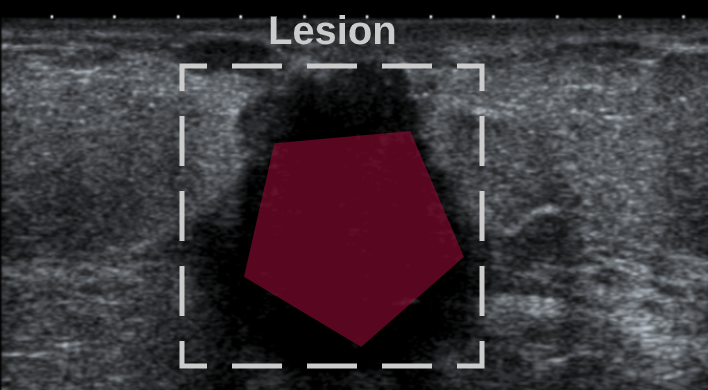
\includegraphics[width=\textwidth]{images/fig004}
\caption{In this work, medical image segmentation is defined as the process of manually draw for boundaries within various modalities of images. The goal of the clinician is to annotate the lesion between the red polygon and the dashed gray square.}
\label{fig:fig004}
\end{figure}
%%%%%%%%%%%%%%%%%%%%%%%%%%%%%%%%%%%%%%%%%%%%%%%%%%%

\subsubsection{Lesion Delineation}
\label{sec:sec004003002001}

Manual annotations (Figure~\ref{fig:fig007}) are very useful to extract features like contours, intersections, shapes (Figure~\ref{fig:fig021}) and image patterns (Figure~\ref{fig:fig022}).
For a proper classification to be integrated into intelligent agents, the tool can be used in the process of lesion delineation and segmentation.
The \ac{AI} algorithm then utilizes this closed contour line information to infer the labels for remaining image elements.
In comparison to early developed work~\cite{calisto2017mimbcdui}, this tool functionality is now reducing the overall annotating process of one lesion to take less user interaction time~\cite{10.1145/3132272.3134111, 10.1145/3399715.3399744}.
However, reaching an appropriate or even perfect segmentation leads space for improvements, which are addressed as future work (Chapter~\ref{chap:chap008}) under this thesis.
In fact, the proposed interactive approach aims at a fast and exact segmentation with knowledge about estimates of the true lesion extent.
During this process, clinicians are providing and generating new information transformed into an important dataset for the \ac{AI} community.

%%%%%%%%%%%%%%%%%%%%%%%%%%%%%%%%%%%%%%%%%%%%%%%%%%%
\begin{figure}[ht]
\centering
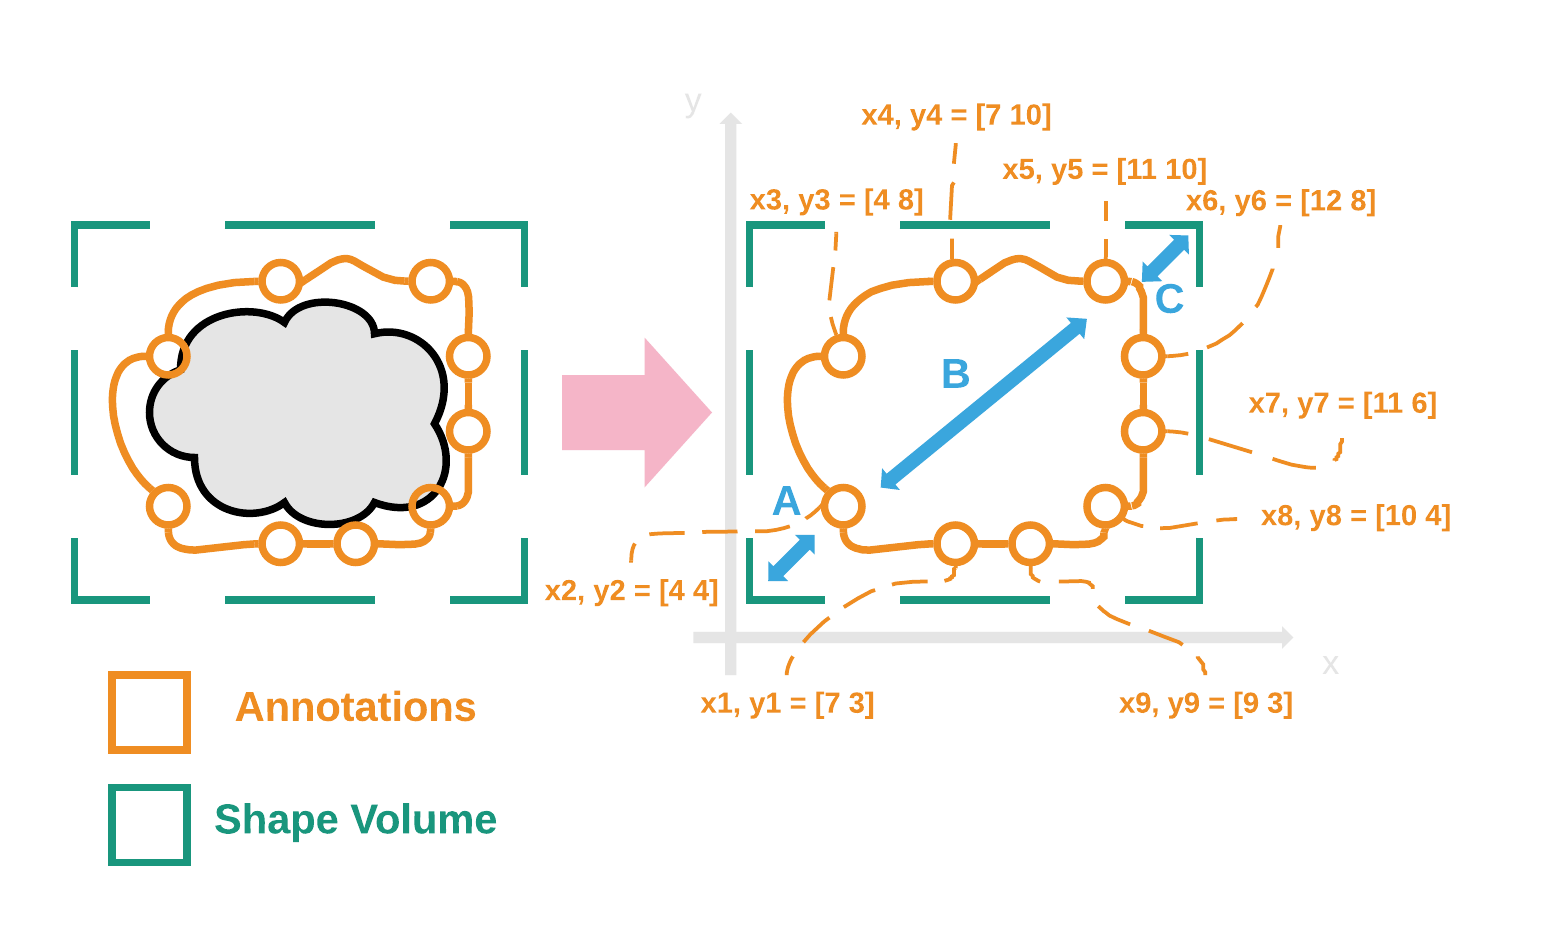
\includegraphics[width=\textwidth]{images/fig007}
\caption{Labels of the Lesions~\cite{nadia2020maivell} - the grey area is the lesion, the yellow represents the annotations taken by the radiologist, the green area represents the shape volume. The image on the right aims to explain how the coordinates are represented. The image on the left aims to explain how the annotations are visually appearing on the screen.}
\label{fig:fig007}
\end{figure}
%%%%%%%%%%%%%%%%%%%%%%%%%%%%%%%%%%%%%%%%%%%%%%%%%%%

In this section, the document explains how the chapter is contributing for the delineation and annotation (Section~\ref{sec:sec004003002002}) of medical images.
Here, the document refers to lesion delineation as the \ac{ROI} area of the lesion which is delineated by a clinician, such as a radiologist.
Further explained (Figure~\ref{fig:fig007}), the document will visually provide the relations between lesion and delineation process.

\subsubsection{Lesion Annotations}
\label{sec:sec004003002002}

In this framework, the user interact with the \ac{UI} making bullet points (Figure~\ref{fig:fig007}), which can be connected ({\it i.e.}, by selecting the {\it 5.2.7. Freehand} functionality for masses) or not ({\it i.e.}, by selecting the {\it 5.2.8. Probe} functionality for microcalcifications), among the contours of the lesion.
Each bullet point is referenced to an \texttt{x} and \texttt{y} pair of coordinates.
The \texttt{x} and \texttt{y} coordinates (Section~\ref{sec:sec004004}) are the position on the image.
With this, it can be measured the ground-truth of the lesion, {\it i.e.}, {\bf Shape Volume} (Figure~\ref{fig:fig007}), and give this information to the \ac{ML} algorithms.
Also, it is now possible to autonomously classify the margins and shapes of masses (Figure~\ref{fig:fig021}), as well as the distribution patterns of calcifications (Figure~\ref{fig:fig022}).

\section{Framework Description}
\label{sec:sec004004}

The goal of this section is to describe the properties and environment characteristics of the framework, having a basic architecture already implemented~\cite{calisto2017mimbcdui}.
As explained before, the purpose of this tool is to work on the \ac{RRR}.
This means that it must be adjusted to a traditional environment (\textit{e.g.}, computer desktop, keyboard and mouse in a dark room), and reliable due to the personal and medical stored information.
Given this situation, a secure but easily accessed framework for clinicians to work with is a requirement.
The herein tool is a distributed system that allows a secure and easy access to information and the manipulation of medical images.
With this kind of image manipulation, in the annotation of the images case, the community can train the \ac{ML} algorithms under control, where the generated data is supervised by both clinicians and researchers in a human-in-the-loop~\cite{10.1145/3306618.3314293} setting.

\subsection{Technologies}
\label{sec:sec004004001}

Concerning the selected technologies, the development decision relies on the available and powerful technologies from the open-source\footnotemark[14] community.
Technological selection criteria was based on robust technologies which will mitigate the limitations of this framework.
For this reason, all the decisions must be balanced.
Thankfully, many selected technologies are heavily used by the open-source community, making it strong and robust for the purpose.
Nevertheless, it must be underlined the following.
Although developments under this work are using open-source technologies for this framework, they will \underline{serve as a {\it proof-of-concept} only} and are serving in this thesis research work.
The purpose of this framework is to suggest new tools to be integrated with several intelligent agents.
The technologies can be changed according to the needs of both domain and environment.
Therefore, a conflict between open-source technologies and this thesis contribution does not exist.

%%%%%%%%%%%%%%%%%%%%%%%%%%%%%%%%%%%%%%%%%%%%%%%%%%%
\footnotetext[14]{The advantage of using an open-source setup is that users can tailor it to their requirements, while proprietary setups are a set configuration of functionalities that cannot be changed. Even when the initial tool does not address a specific need, the community will guide researchers and help them to develop a new tool. In this thesis, an open-source setup was used to enable collaboration of individuals and groups promoting the development of intelligent agents that meet user needs.}
%%%%%%%%%%%%%%%%%%%%%%%%%%%%%%%%%%%%%%%%%%%%%%%%%%%

\subsubsection{Source Code}
\label{sec:sec004004001001}

To maintain the framework, the proposed source code must remain simple and secure.
Moreover, the source must provide functionalities such as storing medical exams, use browsers to run the solution and must be a remote distributed system-prepared.
By choosing where to present the deployed tool, namely in a browser, choosing to use \href{https://www.sciencedirect.com/topics/computer-science/javascript-code}{JavaScript} as the programming language to run and manipulate the medical images made the best option.
With this programming language it is possible to manipulate those \ac{DICOM}~\cite{Trivedi2019} files.
Thereafter, the developed work used a library focused on medical imaging manipulation, \href{https://cornerstonejs.org/}{CornerstoneJS}\footnotemark[15], which be will be explain in detail later.
We will also need to have image visualization for what we use \href{http://vanilla-js.com/}{VanillaJS}\footnotemark[16], which we will also explain in detail later.
In terms of source code, the web application uses \href{https://www.sciencedirect.com/topics/computer-science/javascript-code}{JavaScript}, which is an \href{https://www.sciencedirect.com/topics/computer-science/object-oriented-programming}{\ac{OO}} language, \href{https://www.sciencedirect.com/topics/earth-and-planetary-sciences/document-markup-languages}{\ac{HTML}} and \href{https://www.w3schools.com/css/}{\ac{CSS}} technologies.
This source is powerful and flexible.
Based on this, we are going to use all three of them in this invention as a {\it proof-of-concept}.

%%%%%%%%%%%%%%%%%%%%%%%%%%%%%%%%%%%%%%%%%%%%%%%%%%%
\footnotetext[15]{Comparing to other libraries in the same field, the advantaged point of \href{https://cornerstonejs.org/}{CornerstoneJS} (\href{https://cornerstonejs.org/}{cornerstonejs.org}) is a collection of clear instructions and examples which are available in an intuitive \href{https://docs.cornerstonejs.org/}{library documentation}. Therefore, it can help developers and researchers saving time for developing process of their applications. These links were accessed on the 1st of December, 2020.}
%%%%%%%%%%%%%%%%%%%%%%%%%%%%%%%%%%%%%%%%%%%%%%%%%%%

%%%%%%%%%%%%%%%%%%%%%%%%%%%%%%%%%%%%%%%%%%%%%%%%%%%
\footnotetext[16]{\href{http://vanilla-js.com/}{VanillaJS} is a name that refers to the using plain \href{https://www.sciencedirect.com/topics/computer-science/javascript-code}{JavaScript} without any additional libraries ({\it e.g.}, \href{https://reactjs.org/}{ReactJS}, \href{https://angularjs.org/}{AngularJS}, etc). In this thesis, \href{http://vanilla-js.com/}{VanillaJS} was used to implement the main functionality and handlers for the tool requirements. Again, all of these links were accessed on the 1st of December, 2020.}
%%%%%%%%%%%%%%%%%%%%%%%%%%%%%%%%%%%%%%%%%%%%%%%%%%%

\hfill

\noindent
The JavaScript allows multi-paradigm approaches, such as:

%%%%%%%%%%%%%%%%%%%%%%%%%%%%%%%%%%%%%%%%%%%%%%%%%%%
\begin{enumerate}
\item {\bf Client-Side} Scripting Language - runs on the computer browser;
\item {\bf \ac{OO}} Language - each ``object'' has its attributes and methods;
\item {\bf Interpreted Language} - doesn't need to be compiled;
\item {\bf Imperative} and \textbf{Declarative} - can change the state and show what it's doing but not how it is doing, respectively;
\item {\bf Functional} Language - has mathematical based functions.
\end{enumerate}
%%%%%%%%%%%%%%%%%%%%%%%%%%%%%%%%%%%%%%%%%%%%%%%%%%%

Under this thesis, the current and future developed tools are basing the above list of approaches with respect to JavaScript technologies.
The JavaScript technologies are implemented along with the \href{https://jquery.com/}{JQuery} library for \ac{HTML} manipulation, event handling, and \href{https://github.com/cornerstonejs/dicomParser}{\texttt{dicomParser}}\footnotemark[17] library, because it simplifies the coding.
However, these technologies do not add functionality.
Instead, these technologies are simplifying the code and minimizing it.
What is great for framework maintainability purposes.
The above mentioned approaches are used to develop all tool functionalities.
Such technologies, are giving this work the ability to make visual representations on an easily way.

%%%%%%%%%%%%%%%%%%%%%%%%%%%%%%%%%%%%%%%%%%%%%%%%%%%
\footnotetext[17]{The \href{https://github.com/cornerstonejs/dicomParser}{\texttt{dicomParser}} (\href{https://github.com/cornerstonejs/dicomParser}{github.com/cornerstonejs/dicomParser}) is a lightweight library for parsing \href{http://dicom.nema.org/medical/dicom/current/output/html/part10.html}{DICOM P10} byte streams in modern \href{https://developer.mozilla.org/en-US/docs/Web/Guide/HTML/HTML5}{HTML5} based web browsers. The library is fast, easy to use and has no required external dependencies. These links were accessed on the 1st of December, 2020.}
%%%%%%%%%%%%%%%%%%%%%%%%%%%%%%%%%%%%%%%%%%%%%%%%%%%

According to the current state of the developed framework, a tool was implemented using \href{https://cornerstonejs.org/}{CornerstoneJS}~\cite{urban2017lesiontracker} with a \href{https://nodejs.org}{NodeJS} server.
To populate the framework tool, the user can upload sets of patients' images (Section~\ref{sec:sec002007}) into an \href{https://www.orthanc-server.com}{Orthanc Server}~\cite{Jodogne2018}.
Each patient has three modalities (\ac{MG}, \ac{US}, and \ac{MRI}).
The images can be pre-processed and anonymized (Section~\ref{sec:sec002008}) on the \href{https://www.orthanc-server.com}{Orthanc Server} and then consumed by the developed tool.
This framework is designed as a set of modules that can be reused in other applications.
The \href{https://cornerstonejs.org/}{CornerstoneJS} family of libraries are providing essential functions, such as
(i) image rendering;
(ii) \ac{DICOM} retrieval;
(iii) tool support; and
(iv) interpretation (UI).

\subsubsection{DICOM Server}
\label{sec:sec004004001002}

In this work, it is used the \href{https://www.orthanc-server.com}{Orthanc Server}~\cite{Jodogne2018} distribution to store (Section~\ref{sec:sec002008}) the medical images.
The advantage of using an \href{https://www.orthanc-server.com}{Orthanc Server} is that it is a lightweight server for medical imaging (\ac{PACS}) and it is an open-source project with a free software license.
Also, it has the capability of managing and analyzing all of the contents (Figure~\ref{fig:fig030}), and offers the possibility of visualizing the images in the web browser.

%%%%%%%%%%%%%%%%%%%%%%%%%%%%%%%%%%%%%%%%%%%%%%%%%%%
\hfill
\begin{figure}[ht]
\centering
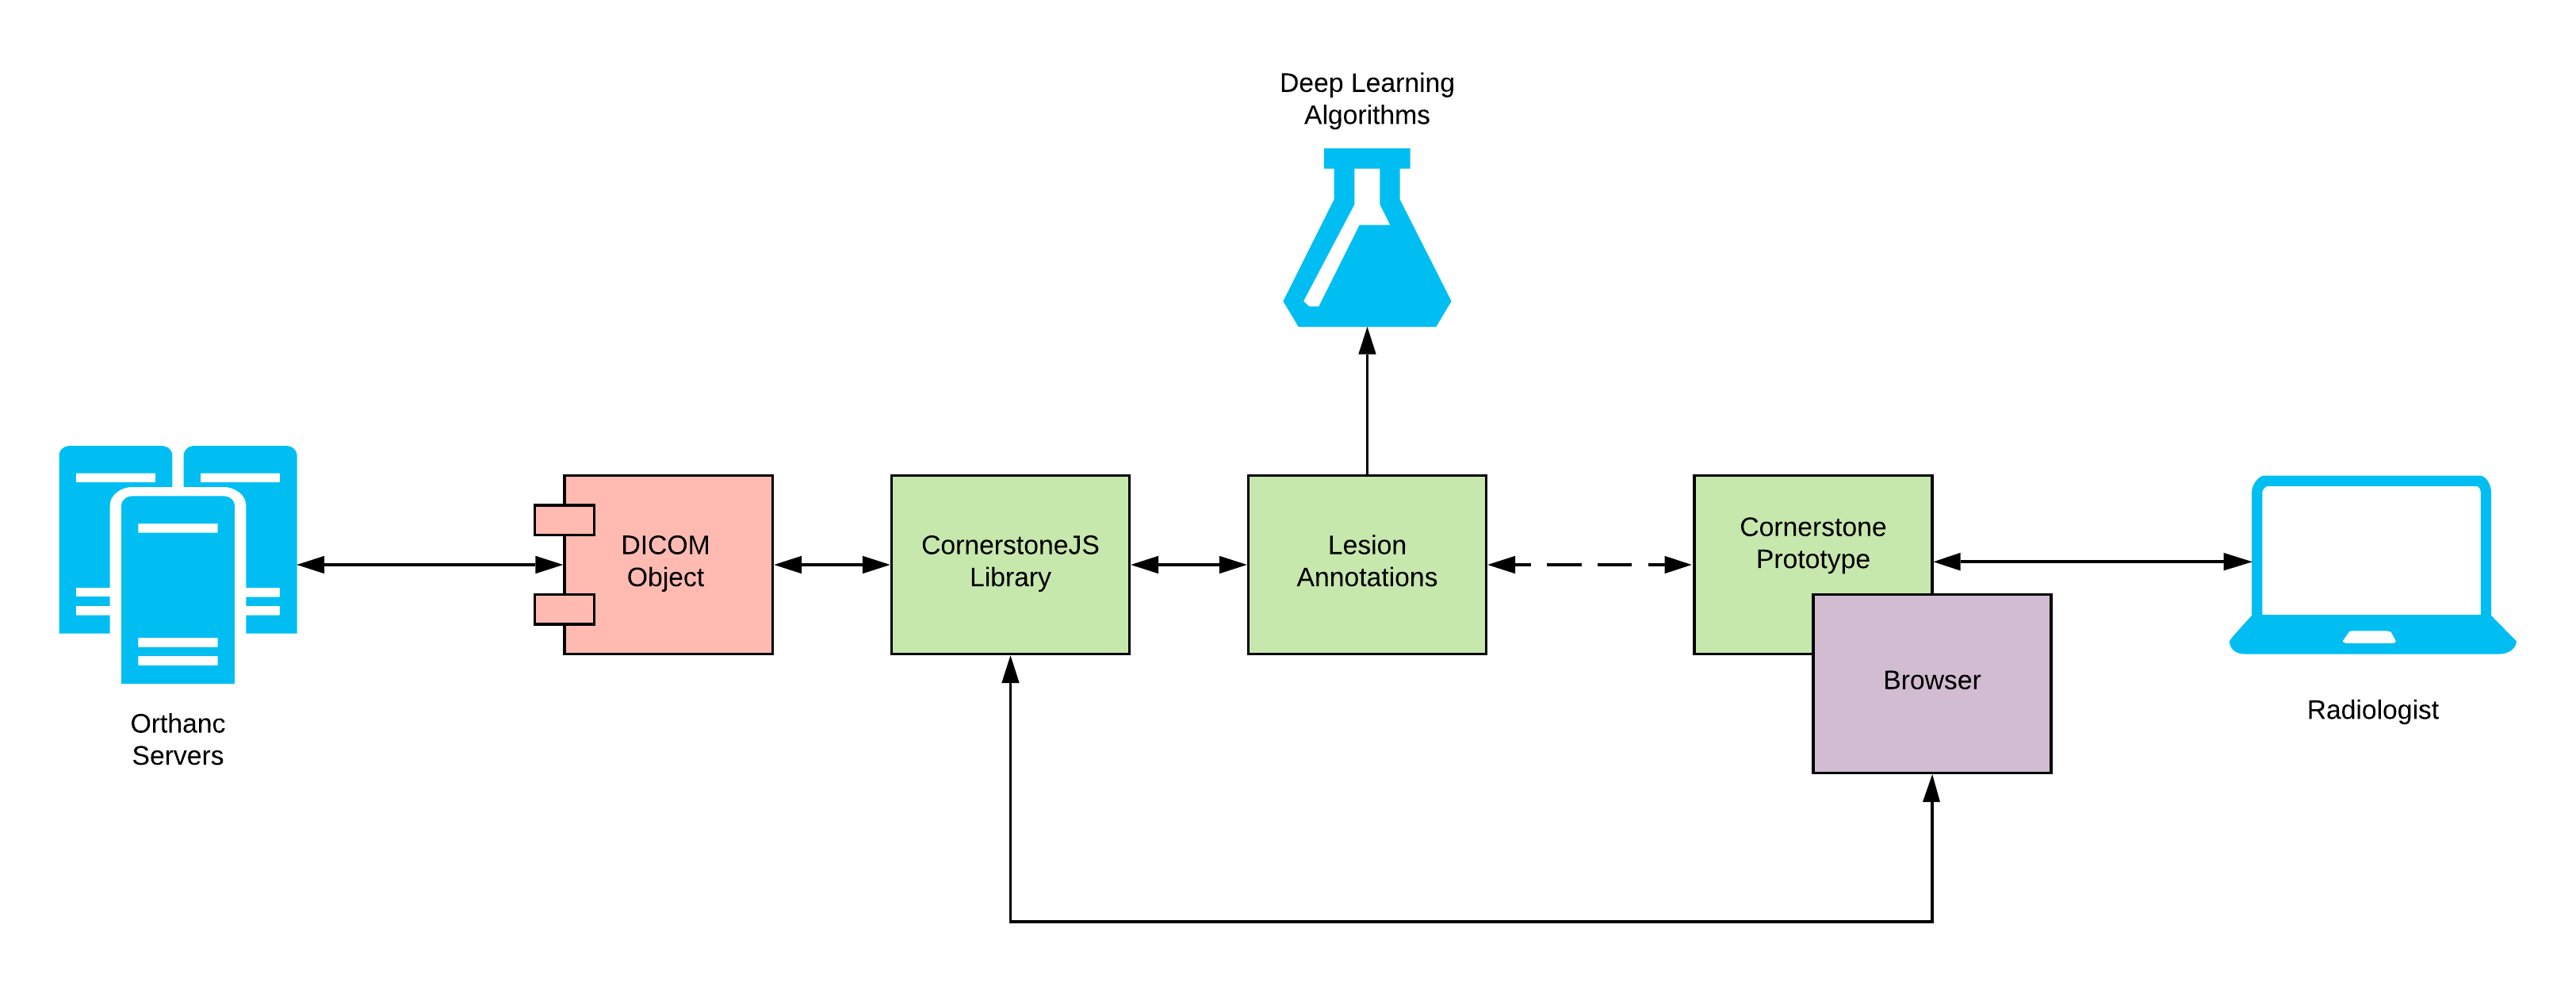
\includegraphics[width=\textwidth]{images/fig030}
\caption{[DOI: \href{http://rgdoi.net/10.13140/RG.2.2.27402.93126}{10.13140/RG.2.2.27402.93126}] Image retrieval~\cite{calisto2019micpuw} from the Orthanc Servers to the DICOM viewer. In this figure, the DICOM viewer is supported by both CornerstoneJS library and Cornerstone Prototype. Now, radiologists can annotate each lesion providing this data to the DL Algorithms.}
\label{fig:fig030}
\end{figure}
\hfill
%%%%%%%%%%%%%%%%%%%%%%%%%%%%%%%%%%%%%%%%%%%%%%%%%%%

A \ac{DICOM} server, like the \href{https://www.orthanc-server.com}{Orthanc Server}, its built-in RESTful API\footnotemark[18] architectures~\cite{6556444}.
It can be used to drive it from external applications.
For instance, the \href{https://cornerstonejs.org/}{CornerstoneJS} set of tools (Section~\ref{sec:sec004004001001}) and originated platforms.
The Orthanc uses several \ac{DICOM} tags from the stored medical images in the \ac{JSON} file format.
The structures for the stored \ac{DICOM} resources are fourfold identifiers:
(1) Patient;
(2) Study;
(3) Series; and
(4) Instance.

%%%%%%%%%%%%%%%%%%%%%%%%%%%%%%%%%%%%%%%%%%%%%%%%%%%
\footnotetext[18]{This REpresentational State Transfer (RESTful API) is a well-documented set of HTTP paths against which it is possible to make HTTP requests with any client tool, such as the standard curl command-line tool. Similarly to \href{https://www.orthanc-server.com}{Orthanc Server}, the RESTful API is served through the embedded Mongoose HTTP server.}
%%%%%%%%%%%%%%%%%%%%%%%%%%%%%%%%%%%%%%%%%%%%%%%%%%%

\subsubsection{Main Server}
\label{sec:sec004004001003}

Similar to other systems~\cite{HOSTETTER2018811}, the proposed framework utilizes a Front-end and a Back-end ecosystem integration for content management, image storage, and image display.
In this section, it is described how the proposed web-based tool (Figure~\ref{fig:fig011}) was created with a Back-end architecture.
By utilizing a common JavaScript framework called NodeJS, the tool was integrated into an existing ecosystem ({\it i.e.}, with CornerstoneJS and Orthanc Server).
The Back-end comprises web server, image storage, content management, and was created with open-source technologies, as well as data storage protocols.

%%%%%%%%%%%%%%%%%%%%%%%%%%%%%%%%%%%%%%%%%%%%%%%%%%%
\begin{figure}[ht]
\centering
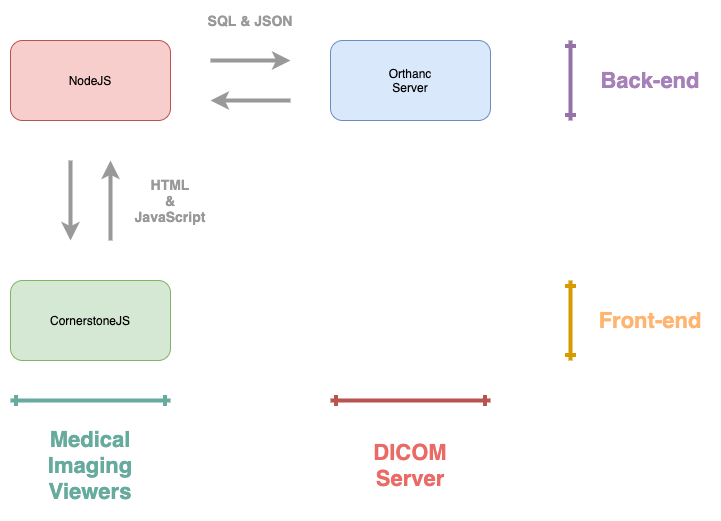
\includegraphics[width=0.90\textwidth]{images/fig011}
\caption{[DOI: \href{https://doi.org/10.13140/rg.2.2.13834.62405}{10.13140/RG.2.2.13834.62405}] Schematic demonstrating both {\bf Front-end} and {\bf Back-end} components of the system with integrated medical imaging solutions. In our solution, we show the use of technologies such as {\bf NodeJS} and {\bf CornerstoneJS} for the {\bf Medical Imaging Viewers}, as well as the {\bf Orthanc Server} for the {\bf DICOM Server} component~\cite{https://doi.org/10.13140/rg.2.2.13834.62405}.}
\label{fig:fig011}
\end{figure}
%%%%%%%%%%%%%%%%%%%%%%%%%%%%%%%%%%%%%%%%%%%%%%%%%%%

Metadata was stored and retrieved using \ac{SQL} and \ac{JSON} databases.
The web server was written in JavaScript using NodeJS, an open-source server-side Back-end implementation of the JavaScript programming language that is powered by V8 JavaScript engine.
NodeJS is a platform built on JavaScript runtime for easy building of fast, scalable network applications on all the operating systems.
Furthermore, NodeJS uses an event-driven, non-blocking \ac{IO} model that makes it lightweight and efficient, suitable for data-intensive real-time applications that run across distributed devices.
As a WebSocket library, NodeJS was used for the WebSocket communication.

The net module, which provides asynchronous network wrapper for creating both \ac{TCP} servers and clients, was used with \ac{IP} interconnections.
The NodeJS server listens on two ports for incoming \ac{DICOM} or WebSocket connections.
By using a \ac{DICOM} server (Section~\ref{sec:sec002007}) as a \ac{PACS} (Section~\ref{sec:sec002008}), the NodeJS server knows what image size to expect from incoming \ac{TCP} connection.
When this data is received, the \ac{DICOM} server sends the image to the web client over WebSocket connection.
This method needs to be followed since, in web browsers, JavaScript does not support access to \ac{TCP}/\ac{IP} communication or \ac{DICOM} protocol.
Making it vital to apply this method.

\subsubsection{Summarizing Medical Imaging Viewers}
\label{sec:sec004004001004}

The developed tool is using CornerstoneJS~\cite{10.1117/12.2513004} as an application (Section~\ref{sec:sec004004001001}) that performs the rendering (Section~\ref{sec:sec004004001001}), the download (Section~\ref{sec:sec004004001002}) and some other functionalities (Section~\ref{sec:sec004003002}) across the images.
In this section (Section~\ref{sec:sec004004001}), all of the above characteristics are discussed and summarized to cover the rendering (Section~\ref{sec:sec004004001001}) and communication (Section~\ref{sec:sec004004001003}) concerns in medical imaging.
Moreover, the thesis is going to use this tool to operate the images (Figure~\ref{fig:fig011}), making use of functionalities (Section~\ref{sec:sec004003001003}) such as zoom, contrast, etc.
The CornerstoneJS library can display interactive medical images (Section~\ref{sec:sec004003001002}) on any modern browser that supports the HTML5 canvas element.
This includes desktops, mobile devices, and tablets.
In short, the library is a zero-footprint viewer enabling access to images on a browser without requiring installation of additional software.
Similar types of online medical imaging systems have been previously reported in the radiology literature~\cite{HOSTETTER2018811}.
Those systems are supporting a full range of standard image viewing and manipulation functions including multimodality viewing with zoom, pan, as well as window and image levels.
Annotation of masses (Section~\ref{sec:sec002004001}) and microcalcifications (Section~\ref{sec:sec002004002}) is also implemented (Section~\ref{sec:sec004003002}), allowing measurements of the lesion types (Section~\ref{sec:sec002004}), such as margins and shapes of masses (Figure~\ref{fig:fig021}), as well as microcalcification types (Figure~\ref{fig:fig022}).
Measurements for the \acp{ROI} where developed, with the ability to draw among lesion masses and to bullet point the calcifications.

\subsection{Annotated Data}
\label{sec:sec004004002}

The proposed solution will enable \ac{ML} communities to organize and promote medical imaging projects.
As result of the generated dataset (Figure~\ref{fig:fig013}), the community can now have access to a tool, creating their own datasets of medical images and annotations, respectively.
With this solution, the community has now a way for the data extraction and structured adjudication (Section~\ref{sec:sec003005}) of lesion annotations among the breast cancer disease.
This data is saved to a set of \ac{JSON} files, one per each patient, where each file has \ac{JSON} objects organized into a standard structure.

%%%%%%%%%%%%%%%%%%%%%%%%%%%%%%%%%%%%%%%%%%%%%%%%%%%
\begin{figure}[htbp]
\centering
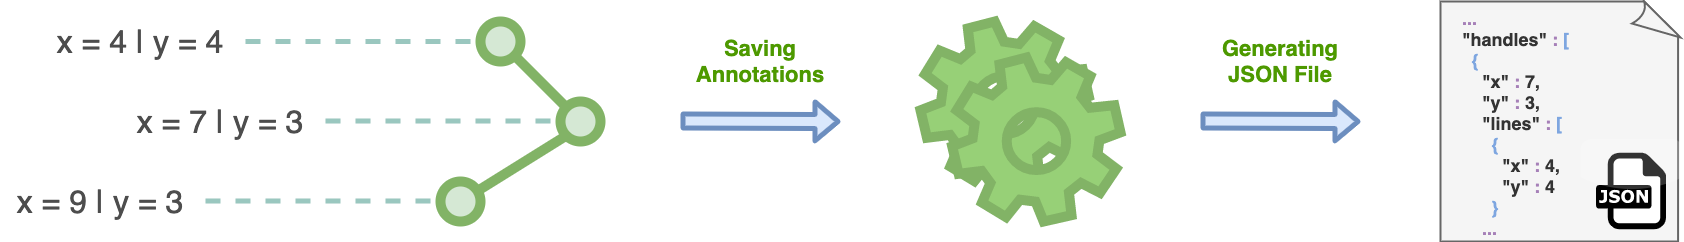
\includegraphics[width=\textwidth]{images/fig013}
\caption{[DOI: \href{https://doi.org/10.13140/rg.2.2.33967.28323}{10.13140/RG.2.2.33967.28323}] Schematic diagram for the annotations flow and JSON file generation~\cite{https://doi.org/10.13140/rg.2.2.33967.28323}. Each bullet point is computed into a pair of coordinates. Then, the set of coordinates is saved as annotations for that patient into the JSON file. Finally, the file is stored on a remote server.}
\label{fig:fig013}
\end{figure}
%%%%%%%%%%%%%%%%%%%%%%%%%%%%%%%%%%%%%%%%%%%%%%%%%%%

Now, the extraction of the latter data (Figure~\ref{fig:fig013}), {\it i.e.}, \ac{JSON} objects, requires specialized knowledge and understanding of the data structure.
Bullet points under the image are the most intuitive form of user input~\cite{10.1145/3132272.3134111, 10.1145/3399715.3399744}.
Clinicians use this technique when transferring knowledge via visual assets on medical images.
Having this in mind, the document can mathematically detail the transformation of these visual assets into data structures of the generated dataset.

The overlaid mask on the visualization of the image ${\bf I}~\in~\mathbb{R}^{w, h}$ to segment, consists of structures called annotations, where $w$ is the width and $h$ is the height of image ${\bf I}$ in pixels.
In every image ${\bf I}$, it is possible to annotate several ${\it i}~\in~\mathbb{N}$ number of lesions.
The set of annotations is made of two structure options for: (1) masses by using the freehand functionality; and (2) microcalcifications by using the probe functionality.
One set of annotations is a tuple ${\bf a}$~=~(${\bf F}$, ${\bf P}$), where $\texttt{F}~=~\{{\bf f}_{1}, {\bf f}_{2}, ...\}$ is made of $\texttt{f}_{i}~\in~\mathbb{R}^2$ subsets and $\texttt{P}~=~\{{\bf p}_{1}, {\bf p}_{2}, ...\}$ is made of $\texttt{p}_{i}~\in~\mathbb{R}$ subsets.
Each bullet point is a tuple of coordinates ${\bf c}$~=~($\texttt{x}$, $\texttt{y}$), where $\texttt{x}~\in~\mathbb{R}$ describes horizontal \texttt{x} position and $\texttt{y}~\in~\mathbb{R}$ describes vertical \texttt{y} position of ${\bf c}$ in an {\bf I} image with a $w$ and $h$ size.
Freehand annotations are bullet points ${\bf f}_{i}$~=~($\texttt{s}_{i}$, $\texttt{t}_{i}$), where each child $\texttt{t}_{i}~\in~\mathbb{R}^2$ has a parent $\texttt{s}_{i}~\in~\mathbb{R}^2$ and is connected by a line.
A child is a $\texttt{t}_{i}$ of target coordinates and a parent is a $\texttt{s}_{i}~\in~\mathbb{R}^2$ of source coordinates.
The process ends when the clinician intersects the last bullet point ${\bf f}_{n~-~1}$ for ${\it n}~\in~\mathbb{N}$ into the first ${\bf f}_{0}$ bullet point.
Probes ${\bf p}_{i}$~$\supset$~$\texttt{c}_{i}$ are bullet points with simple plain ({\it i.e.}, with no child/parent logic) structures, meaning that a probe is simply a coordinate.
As follows, this section is explaining the annotations data structure for the \ac{JSON} files generation from user interactions.

By selecting (Section~\ref{sec:sec004003001003}) the {\it 5.2.7. Freehand} ({\it i.e.}, the \texttt{freehand} tag of the \ac{JSON} file) or the {\it 5.2.8. Probe} ({\it i.e.}, the \texttt{probe} tag of the \ac{JSON} file) feature (Figure~\ref{fig:fig008}), the tool will generate an array of objects.
Each object is a list of variables, which are referencing the sate, {\it i.e.}, \texttt{visible} and \texttt{active}, of the annotations.
The last variable, {\it i.e.}, \texttt{handles}, is the array of objects with the coordinates, {\it i.e.}, \texttt{x} and \texttt{y}, of the annotations.
Moreover, each \texttt{handles} object has another three state variables: (1) \texttt{highlight}; (2) \texttt{active}; and (3) \texttt{lastFlag}.
Finally, each \texttt{handles} object has also an object of \texttt{lines}.
The \texttt{lines} are sets of objects where each object ({\it i.e.}, child coordinates) represents all \texttt{x} and \texttt{y} coordinates of a parent.
However, in this solution each \texttt{x} and \texttt{y} parent coordinate have one, and only one, associated \texttt{x} and \texttt{y} child coordinate.
Because of that, we called this variable as \texttt{lines}, since the variable refers to the visually connected line between child/parent coordinates.

\noindent
The following snippet, shows a possible sample of a \ac{JSON} source by following the Figure~\ref{fig:fig007} example:

\hfill

\begin{lstlisting}[language=json,firstnumber=1]
"freehand":[ 
  { 
    "visible":true,
    "active":false,
    "handles":[ 
      { 
        "x":7,
        "y":3,
        "highlight":true,
        "active":true,
        "lastFlag":false,
        "lines":[ 
          { 
            "x":4,
            "y":4
          }
        ]
      },
      ...
      { 
        "x":9,
        "y":3,
        "highlight":true,
        "active":true,
        "lastFlag":false,
        "lines":[ 
          { 
            "x":7,
            "y":3
          }
        ]
      }
    ],
    "highlight":false
  }
]
\end{lstlisting}

The value of \texttt{freehand}, \texttt{probe}, \texttt{handles} and \texttt{lines} must be one array of objects. The values of \texttt{visible}, \texttt{active}, \texttt{highlight} and \texttt{lastFlag} must be boolean ({\it e.g.}, \texttt{true} or \texttt{false}). Finally, the values of \texttt{x} and \texttt{y} coordinates must be {\it integers} or {\it floats}.

\subsection{System Architecture}
\label{sec:sec004004003}

Hereinafter, the section is briefly explaining how diagnose and lesion annotations are performed (Figure~\ref{fig:fig012}) by a clinician using the proposed framework.
A more detail explanation will be given at the end of this section.
First of all, clinicians acquire the patient images and perform a medical exam that is then stored as a \ac{DICOM} file (Section~\ref{sec:sec002007}) on the \ac{DICOM} server (Section~\ref{sec:sec004004001002}).
Thereafter, the clinician will open the browser and an Orthanc connection, signing-in with medical credentials (Section~\ref{sec:sec004004001003}).

%%%%%%%%%%%%%%%%%%%%%%%%%%%%%%%%%%%%%%%%%%%%%%%%%%%
\begin{figure}[ht]
\centering
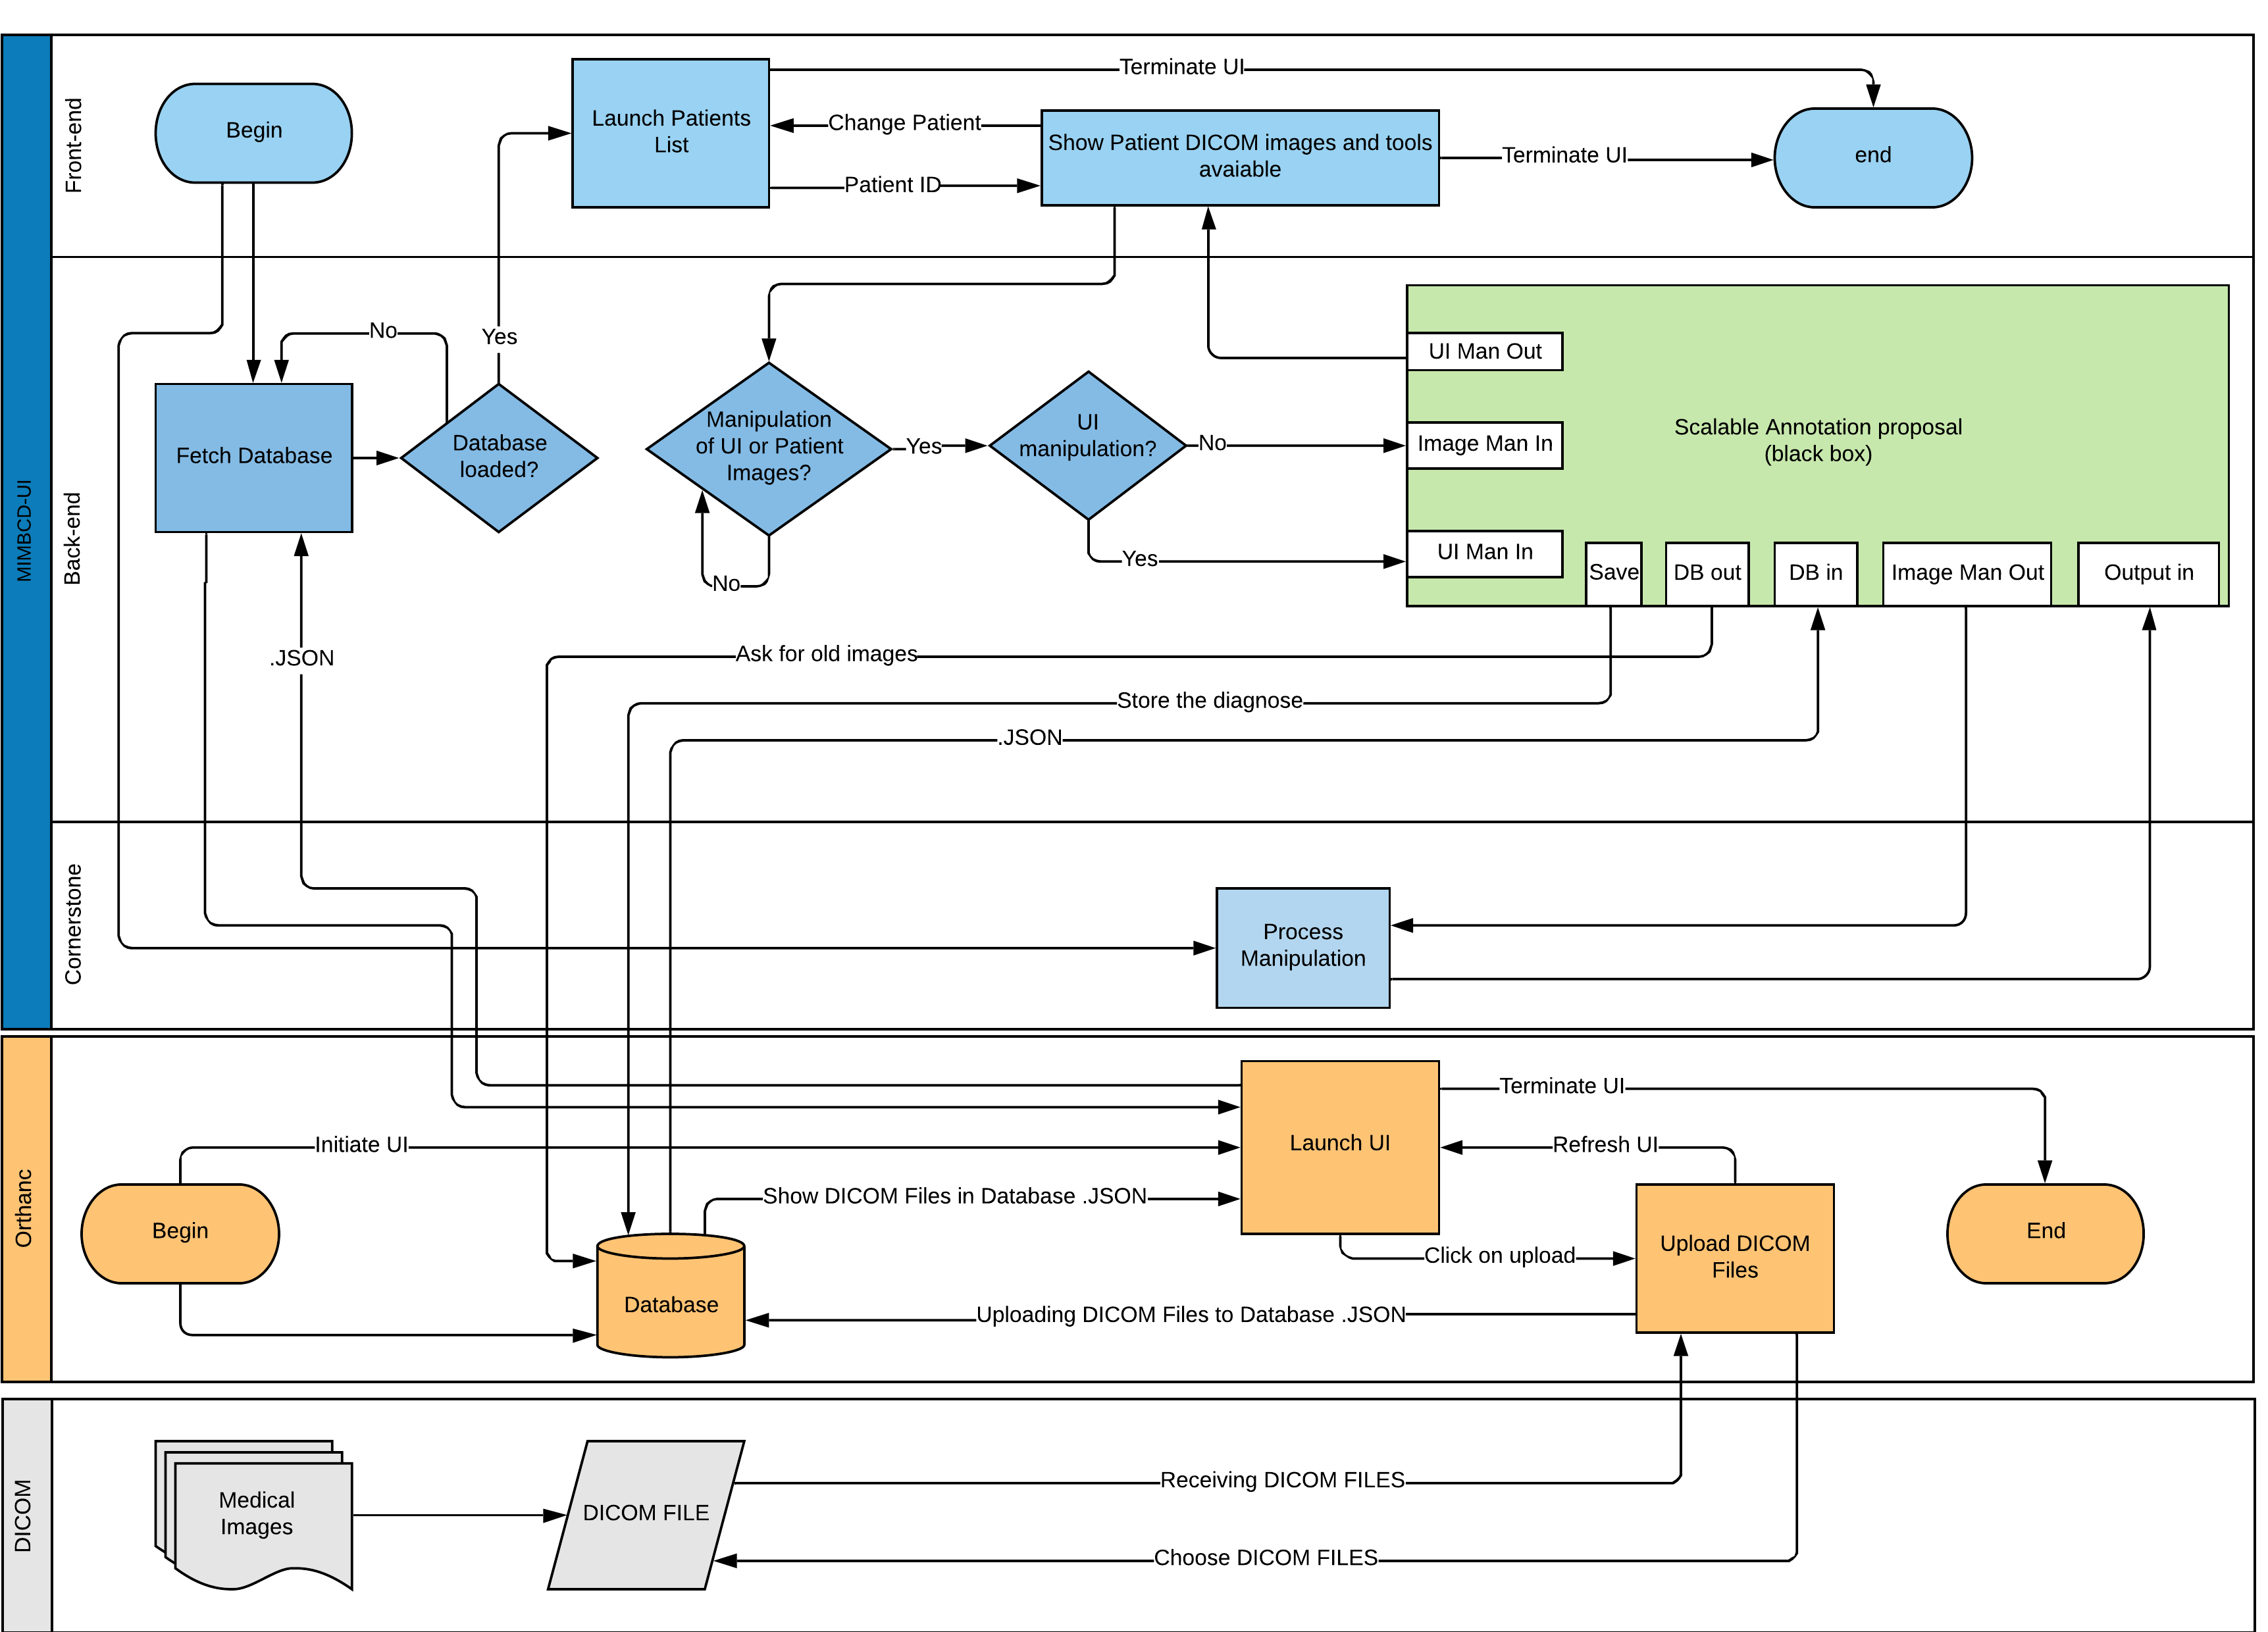
\includegraphics[width=\textwidth]{images/fig012}
\caption{[DOI: \href{https://doi.org/10.13140/RG.2.2.16601.47209}{10.13140/RG.2.2.16601.47209}] System architecture of the invention with a black box of scalable interactions~\cite{hugo2020si, lencastre2020msia}.}
\label{fig:fig012}
\end{figure}
%%%%%%%%%%%%%%%%%%%%%%%%%%%%%%%%%%%%%%%%%%%%%%%%%%%

In the end, the connection is completed, the browser will request (Section~\ref{sec:sec004004001001}) available images to the server and present (Section~\ref{sec:sec004003001}) them through the \ac{UI}.
By opening a patient case (Section~\ref{sec:sec002007}) the clinician will visualize the \ac{DICOM} files and manipulate (Section~\ref{sec:sec004003001001}) those files using the available tools.
Finally, after analysing the medical exams, clinicians will diagnose the patient.

Now, the Orthanc Server is launched and the database is ready and will stay on standby, waiting for requests.
All available patient images are requested by the framework to the Orthanc Server and if the response given is successful, a \ac{JSON} file is received.
After a successful database fetch, it is reported back to the clinician the list of patients available for diagnose.
The clinician will now choose a patient to diagnose, and the \ac{UI} will show (Figure~\ref{fig:fig003}) all the available images on the left side of the screen.

\section{Discussion}
\label{sec:sec004005}

With the hype of \ac{AI} methods, such as \ac{ML} and \ac{DL} algorithms, intelligent agents are closer to the \ac{RRR} than ever~\cite{He2019, DANA2020541}.
This proximity, makes highly relevant to the \ac{ML} community, whom is showing interest on solutions for the generation of datasets among medical imaging.
Datasets are generated by an oracle ({\it e.g.}, clinicians, radiologists, etc), having more supervised data~\cite{MAICAS2019101562, 10.1007/978-3-030-59719-1_44} to train their methods.
A greater human-centered approach is requiring sufficient validation and continuous monitoring of emerging \ac{AI} tools, as well as the available data from breast cancer screening.
That said, \ac{NHS} are on the need for frameworks, such as the one developed under this thesis, to a continuous monitoring and re-calibration of these \ac{AI} tools.

\subsection{Stakeholders}
\label{sec:sec004005001}

Several of these \ac{AI} tools have garnered medical regulatory approval within multiple countries, including Portugal and other \ac{EU} members~\cite{pesapane2018artificial, vayena2018machine}.
With the approval of this medical regulations, these frameworks and tools can now be marketed for clinical use directly to stakeholders such as clinicians, physicians and radiologists.
However, key stakeholders, including major payers, service providers, and women undergoing routine screening, need convincing evidence that these new tools can reliably improve screening performance beyond current practice standards.
For instance, by reducing the numbers of \ac{FP} and \ac{FN} values.

Given the ``black box'' nature of \ac{AI} algorithms, there are a number of unique challenges in the process of algorithm validation and stakeholder acceptance.
There is a myriad of ethical, social, political and technical issues regarding \ac{AI} algorithm validation.
Thus, there is some work to do regarding major pressing issues in validating those methods from the perspective of regulatory agencies, organizations with imaging data, and \ac{AI} researchers.
In the research developed under this thesis, the work already formulated two collaborative protocols with two main Portuguese clinical institutions: (1) \href{https://hff.min-saude.pt/}{Hospital Fernando Fonseca}; and (2) \href{http://www.ipolisboa.min-saude.pt/}{IPO Lisboa}.
The purpose of these protocols is the interchange of data and knowledge.
In this work, several other protocols are being formalized.
However, there already exists (Chapter~\ref{chap:chap005}) various collaboration agreements for user testing purposes in a total of nine clinical institutions.

\subsection{Technology Transfer}
\label{sec:sec004005002}

Clinicians, such as radiologists, are key stakeholders for several current \ac{AI} challenges~\cite{pesapane2018artificial}.
They do that by creating high quality training datasets, but also by doing the interpretation of obtained results, and definition of clinical tasks to address.
Indeed, they represent the final user of these technologies.
For that reason, radiologists point of view and feedback are crucial to optimize the use of \ac{AI}-based solutions, such as proposed framework.

Concerning these developments, part of the thesis is solving five key problems:
(a) providing a tool to improve the curation of sufficient image data on \ac{AI} algorithm development and evolution supporting medical imaging;
(b) promoting the generation of medical imaging datasets to be compared by several \ac{AI} methods among the literature;
(c) also providing a tool for clinicians to collaborate each other on a remote and distributed fashion;
(d) bringing together several medical imaging modalities on a multimodality visualization strategy; and
(e) offering the opportunity for clinicians to diagnose each patient with the above characteristics and in the same time generating a dataset while simply interacting with the \ac{UI}.

By solving these five key points, the thesis is addressing several opportunities with the proposed solution, as well as in further inventions.
Actually, \ac{AI} is driving factor behind market growth in medical imaging.
By 2023, \ac{AI} in medical imaging\footnotemark[19] will become a \$2 billion industry.
Making it vital to have a solution, as the one proposed in this thesis, to solve those five problems.

\footnotetext[19]{These claims (\href{https://www.signifyresearch.net/medical-imaging/ai-medical-imaging-top-2-billion-2023/}{signifyresearch.net/medical-imaging/ai-medical-imaging-top-2-billion-2023}) are present in the ``\href{https://www.signifyresearch.net/medical-imaging/ai-medical-imaging-top-2-billion-2023/}{AI in Medical Imaging to Top \$2 Billion by 2023}'' online articled. The article was published on 2nd of August, 2018, and accessed on 2nd of December, 2020. Internet connection is required.}

\section{Conclusions}
\label{sec:sec004006}

In this document, a new method and process supported by an interactive \ac{UI} of a framework platform is proposed.
More precisely, the purpose of this \ac{UI} is to generate a standardized dataset of medical imaging annotations, while initially supporting the future data curation (Section~\ref{sec:sec006004004}) described bellow.
Across the domain of breast cancer, it was adopted a multimodality visualization strategy ({\it i.e.}, \ac{MG}, \ac{US} and \ac{MRI}) for the production of a qualified datasets.
In the end, clinicians are fostering to share and have a collaborative evaluation by developing a distributed, as well as remote accessible framework.

From the beginning of the document (Section~\ref{sec:sec004002}), it is explained how the above framework will provide a solution on the clinical domain.
With this proposed framework (Section~\ref{sec:sec004004}), the document guarantee the detailed requirements to design the final tool.
In the end, the outputs (Section~\ref{sec:sec004004}) of proposed solution will reduce healthcare costs, enabling medical-error mitigation, while improving the patient's healthcare.
Such, is achieved by various embodiment items of this thesis, discussing (Section~\ref{sec:sec004005}) in detail the impact of it.
The properties and environment characteristics, also underline the contextual description, and how it will be addressed to workflow on the \ac{RRR}.